
\chapter{基于三阶相关相位恢复的彩色成像方法}

透过复杂散射介质或在介质内部的光学成像对于生物医学应用来说是一项艰巨的挑战。其根本问题在于,通过散射介质的光会被强烈散射并扩散成复杂的散斑图案,使物体的颜色和空间信息变得无序混乱\cite{Freund1988,goodman_speckle_2007,bertolotti_non-invasive_2012,katz_non-invasive_2014,Yllmaz2019}。
在散射介质成像的领域中,许多方法已被证明能够克服或利用散射效应\cite{newman_imaging_2016,godara_adaptive_2010,katz_looking_2012,larson_water-soluble_2003,liu_imaging_2011,paniagua-diaz_blind_2019},例如自适应光学\cite{godara_adaptive_2010}、波前整形\cite{katz_looking_2012}、相关成像\cite{bertolotti_non-invasive_2012,katz_non-invasive_2014}、多光子荧光成像\cite{liu_imaging_2011,larson_water-soluble_2003}、鬼成像\cite{paniagua-diaz_blind_2019}和光学相干断层扫描成像\cite{park_full-field_2014}。

同时,通过散射介质进行的彩色成像\cite{conkey_color_2012,leung_acousto-optic_2013,sahoo_single-shot_2017}在对深层组织的非侵入性成像和其他生物医学应用方面扮演着重要的角色,进一步的发展将有利于生物医学应用。随着空间光调制器技术的发展,利用波前整形技术实现了透过散射介质实现彩色成像\cite{leung_acousto-optic_2013,sahoo_single-shot_2017}。
然而,波前整形技术耗时较长,需要对众多像素或者模式进行逐个优化,难以在非入侵的情况下实现波前优化整形。20017年,新加披学者Sahoo等人\cite{sahoo_single-shot_2017}利用光学光谱点扩散函数(Spectral Point Spread Function, sPSF)\cite{Freund1988,goodman_speckle_2007}的去相关性,通过去卷积技术,实现了透过散射介质的彩色成像和光谱成像。
然而,该方法受到光谱去相关带宽的和去卷积计算的限制,仍然存在以下缺点:(\romannum{1})需要对系统的sPSF进行标定;(\romannum{2})成像质量对光学系统稳定性要求极其苛刻。因此,在不标定系统sPSF的情况下,通过传统的彩色成像技术实现散射介质的彩色成像仍然是一个巨大挑战。

在前面章节中,我们对散斑相关成像的方法进行了阐述,并进行了相关实验验证,实验证明了基于OME的散斑相关成像方法能够有效的实现对隐藏目标的成像。该方法的核心思想为:通过计算散斑的自相关$I \bigstar I$,移除掉系统PSF的影响,根据维纳辛钦定律进而获得隐藏目标的傅里叶振幅信息。以恢复隐藏目标的傅里叶振幅信息为支撑,利用相位恢复算法进而实现了隐藏目标的的傅里叶相位信息猜测,实现了隐藏目标的成像。
常见的相位恢复算法需要尝试多次的随机初始猜测,才能较好的恢复图像,但是该方法难以保证正确的恢复隐藏目标的方向信息。当所恢复的隐藏目标方向信息不能保证时,对于透过散射散射介质的彩色成像造成了更大困难。我们是否能够找到恰当的相位恢复算法,确定性的恢复目标,进而实现透过散射介质的彩色成像?

在本章中,我们提出了一种基于三阶相关相位恢复的透过散射介质的彩色成像方法。首先,我们证明了三阶相关相位恢复技术的基本理论;其次,我们通过仿真和实验的方式验证了基于三阶相关相位恢复的散射成像有效性;最后,我们通过实验的方式验证了基于三阶相关相位恢复的透过散射介质的彩色成像方法的有效性。与其他相位恢复技术相比,该相位恢复技术可以保留隐藏目标的方位信息,无需额外步骤或更多先验信息去实现透过散射介质的彩色成像。此外,我们的方法有可能实现透过散射介质的光谱成像。

\section{基于三阶相关相位恢复算法的彩色像基本理论}

首先,我们对本章将要进行的彩色成像理论进行简单陈述。该散射成像方法可以简单理解为:即从分别获取RGB三通道的图像,然后合成彩色图像。RGB三通的的图像信息如何获取?我们可以通过彩色相机或者通过添加滤波片的形式进行分别获取。当分别获取RGB通道的散斑后,我们需要分别对单个散斑进行处理,即分别从散斑中获取隐藏目标的傅里叶振幅信息和相位信息。当分别获取恢复RGB通道后的图像后,我们进行相应的图像合成,基本原理如图\ref{fig:4.1}所示。在图\ref{fig:4.1}中,$P_1$,$P_2$和$P_3$分别表示所获取的不同通道的散斑,$P_1^{\prime}$,$P_2^{\prime}$和$P_3^{\prime}$表示分别从$P_1$,$P_2$和$P_3$中所恢复的隐藏目标信息。
然后,将$P_1^{\prime}$,$P_2^{\prime}$和$P_3^{\prime}$合成最终的彩色图像$P$。

\begin{figure}[htp]
	\centering
	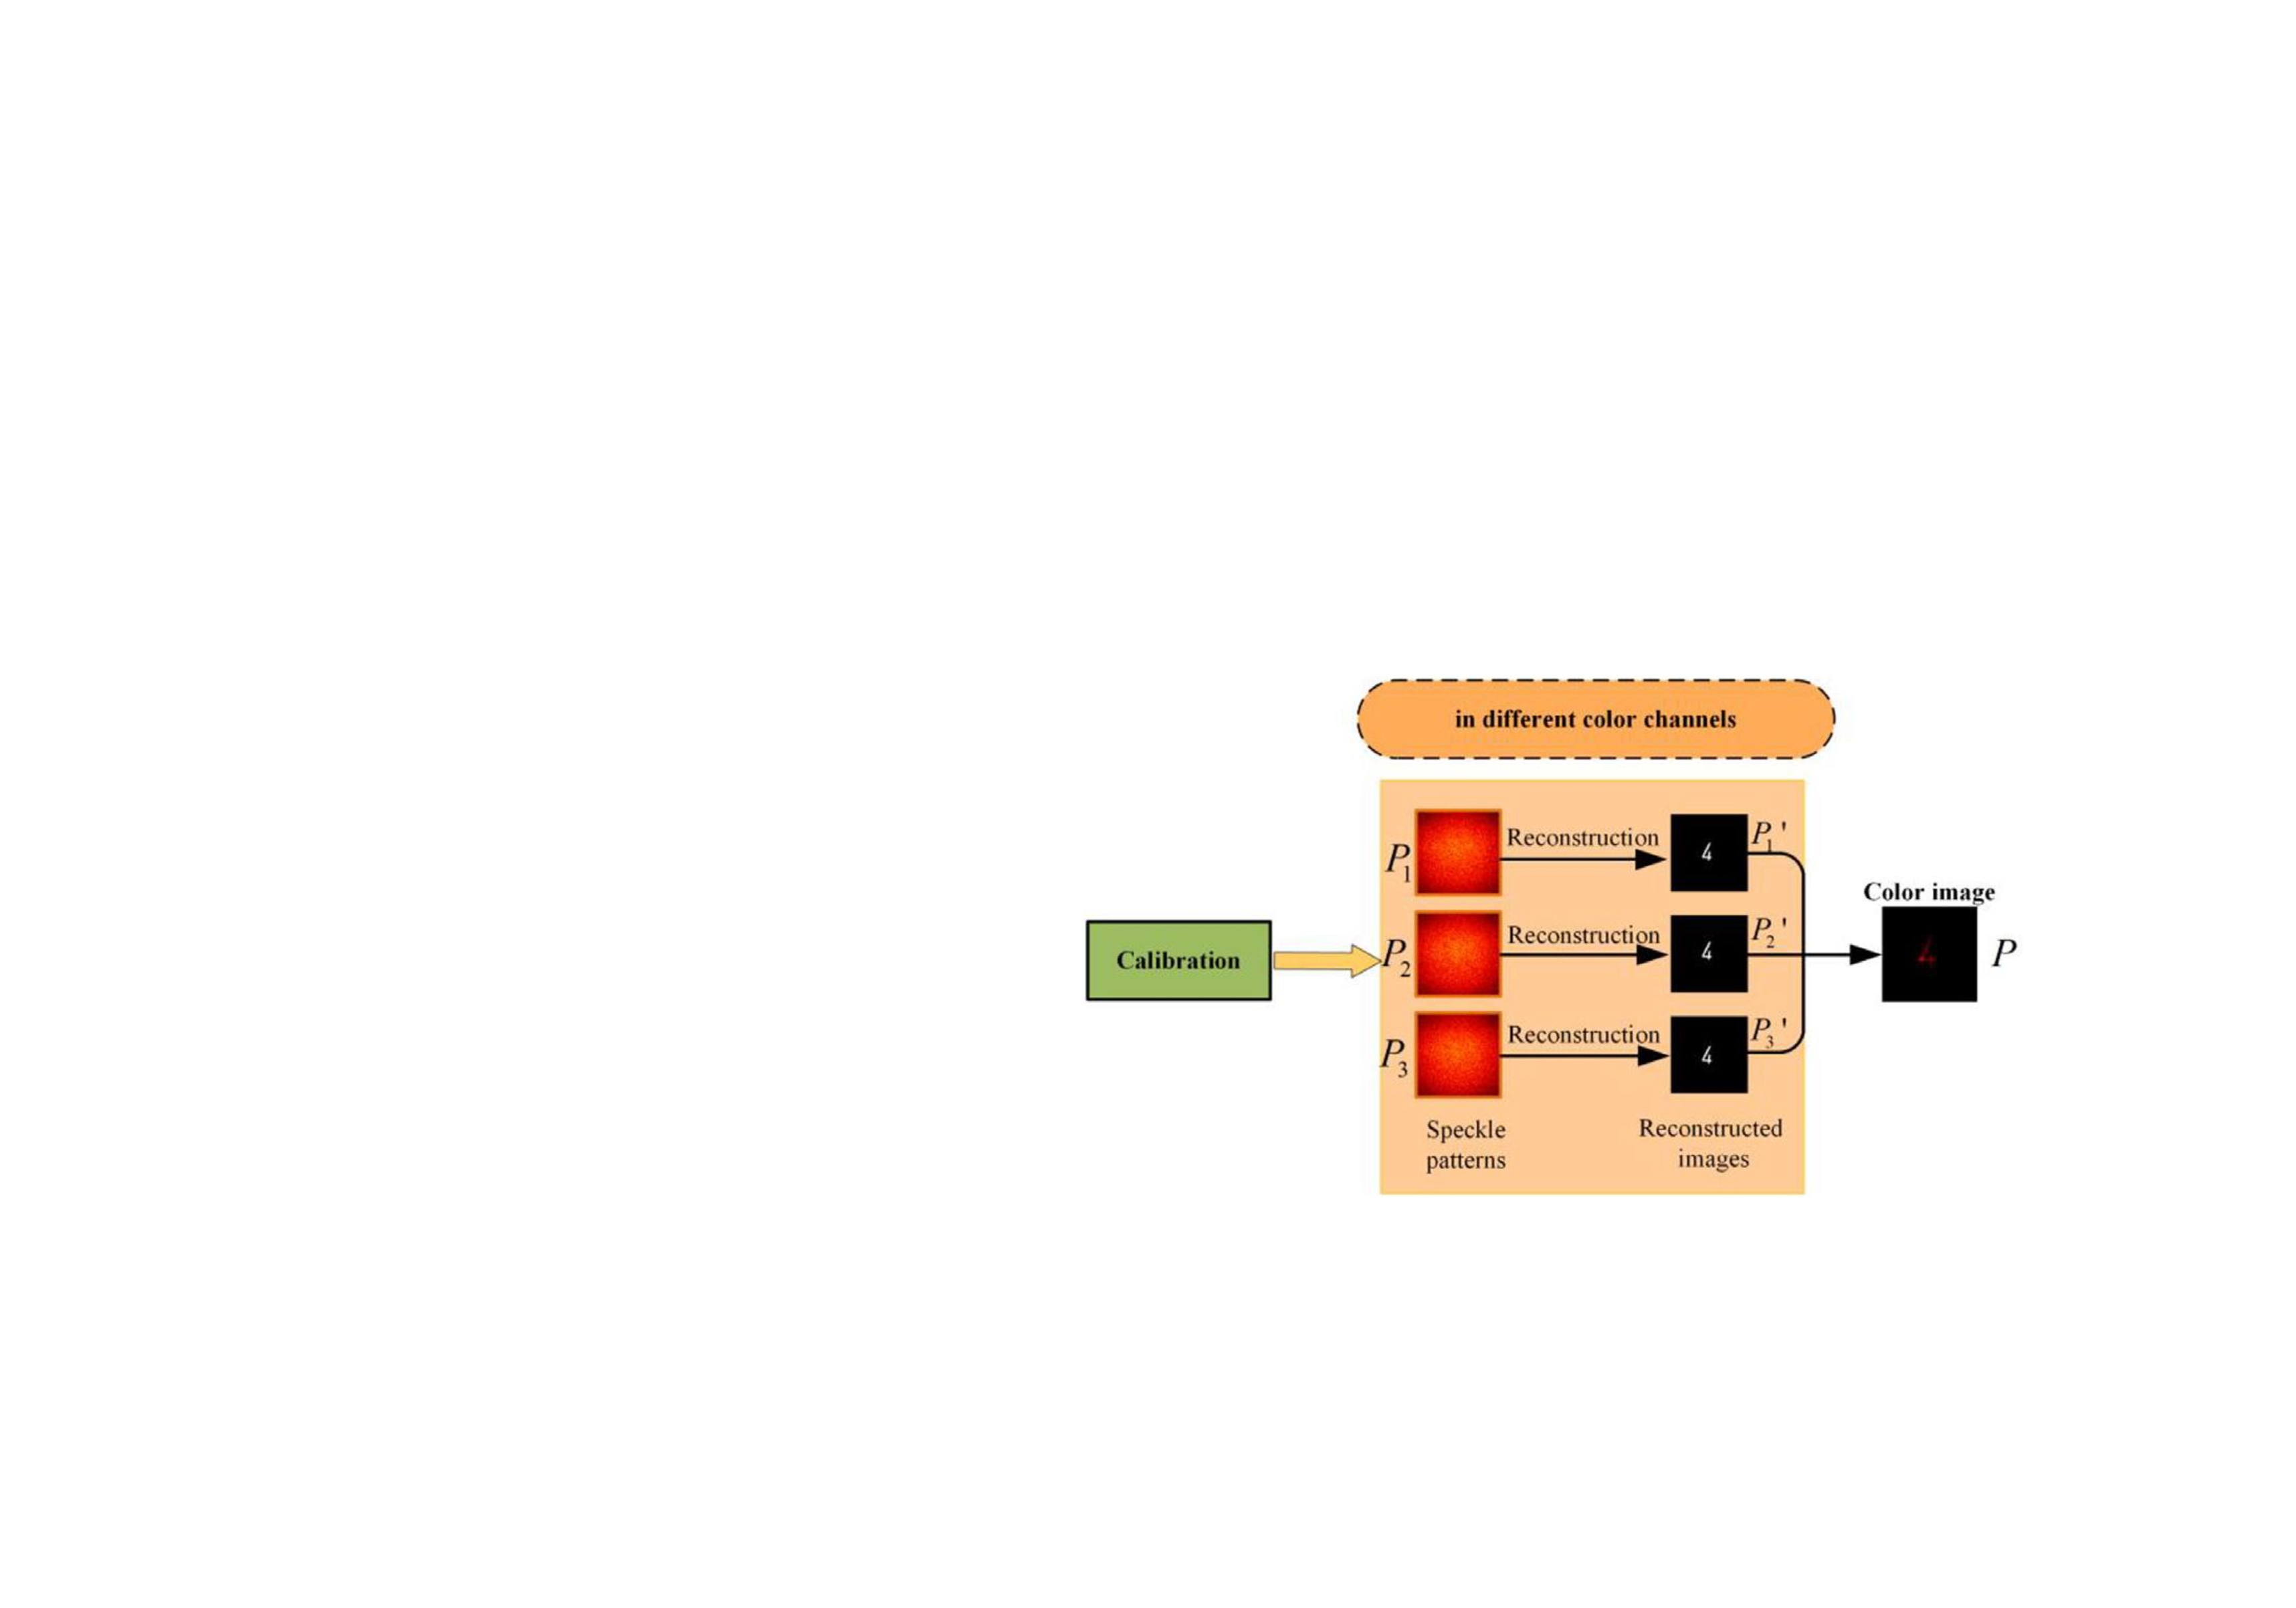
\includegraphics[scale=0.45]{C4.fig1}
	\caption{透过散射介质彩色成像的基本原理}
	\label{fig:4.1}
\end{figure}
在最终合成彩色图像前,如何从单帧散斑中恢复隐藏目标的信息并保存目标的方向信息,如图\ref{fig:4.2}所示,我们将在接下来部分进行详细介绍。
\begin{figure}[htp]
	\centering
	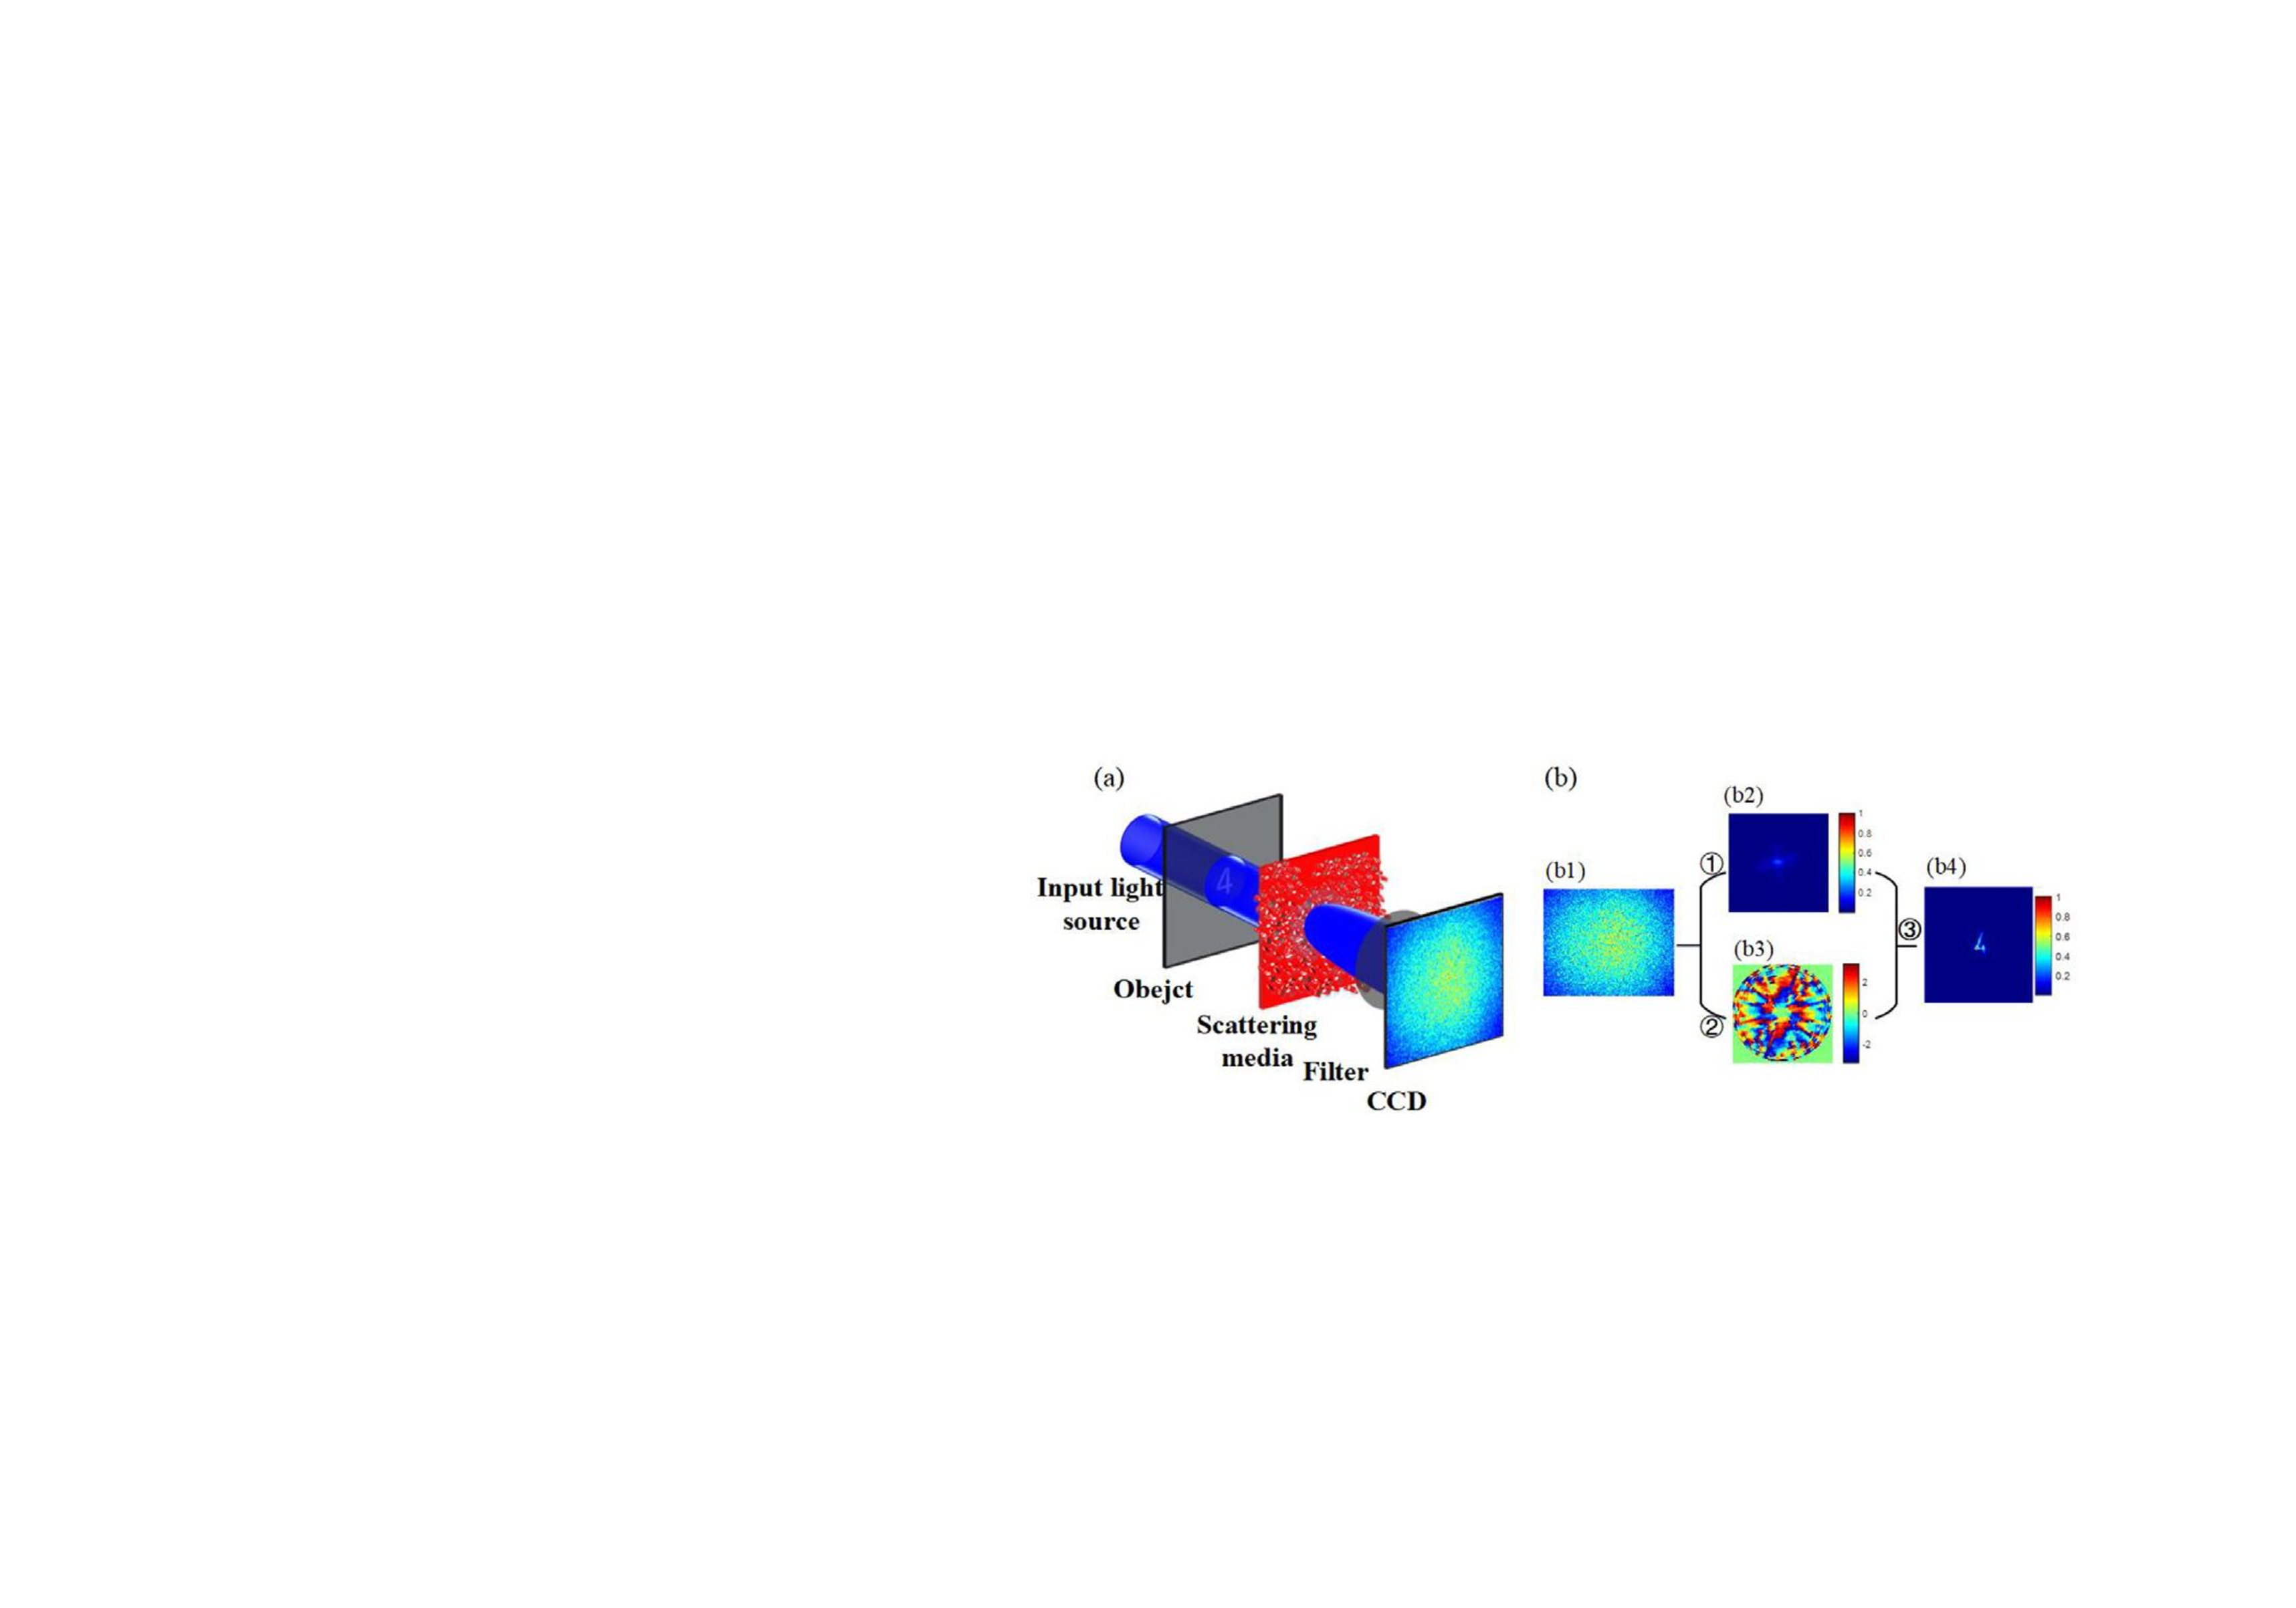
\includegraphics[scale=0.50]{C4.fig2}
	\caption{单帧的透过散射介质成像示意图}
	\label{fig:4.2}
\end{figure}
单帧的透过散射介质成像原理。图\ref{fig:4.2}(a)为实验装置示意图:一束非相干光照亮物体,来自物体的透射光照亮散射介质,最终在CCD上产生散斑图案。图\ref{fig:4.2}(b)为图像恢复流程:(b1)为散斑图案;(b2)为物体的傅立叶振幅; (b3)物体的傅立叶相位和(b4)所恢复的物体图像。其中,{\large \textcircled{\normalsize 1}}表示自相关过程,{\large \textcircled{\normalsize 2}}表示三阶相关相位恢复过程,{\large \textcircled{\normalsize 3}}表示逆傅立叶变换过程。

\subsection{振幅恢复}
在散射介质光学效应区域内时,系统的PSF具有空间平移不变性,所以系统的成像模型可以卷积形式表示:

\begin{equation}
\begin{aligned}
    I &= (O*S)\\
      &= \iint O(x)*S(x) \mathrm{d}{x}
\end{aligned}
\label{eq:4.1}
\end{equation}
其中,$*$表示卷积符号,$I$表示相机所接收到的散斑强度图像,$O$表示目标和$S$表示系统的PSF。

然后通过计算所获得的相机强度散斑图案的自相关,可以获得目标图案的自相关,如公式(\ref{eq:4.2})所示:

\begin{equation}
\begin{aligned}
    I \bigstar I  &= \iint O(x)*S(x) \mathrm{d}{x} \bigstar \iint O(x)*S(x) \mathrm{d}{x} \\
		              & \cong  (O \bigstar O)
\end{aligned}
\label{eq:4.2}
\end{equation}其中,$\bigstar$表示自相关运算。

根据维纳辛钦定理可知,物体的自相关为其物体的功率谱。因此,我们可以通过傅里叶变换的形式,从物体的自相关中恢复物体的傅里叶振幅信息$\mid \mathcal{F}(O) \mid $,如公式(\ref{eq:4.3})所示:
\begin{equation}
\begin{aligned}
   \mid \mathcal{F}(O) \mid \cong \sqrt{\mathcal{F}(I \bigstar I)}
\end{aligned}
\label{eq:4.3}
\end{equation}其中,$\mathcal{F}$表示傅里叶变换运算。

\subsection{相位恢复}

2016年吴腾飞等人\cite{wu_single-shot_2016}受到天文成像的启发,将三阶相关的相位恢复算法引入到散斑自相关成像技术中,三阶相关的相位恢复算法流程如图\ref{fig:4.3}所示,其中,(a)为散斑图案;(b)为子散斑图案(滤波后);(c)为来自第$m$个子散斑图案的一维信号的三阶相关相位;(d)所恢复物体的最终傅立叶相位。( $\theta$ 表示Radon变换的角度,在(b)和(d)中用红色双箭头标记)。

\begin{figure}[htp]
	\centering
	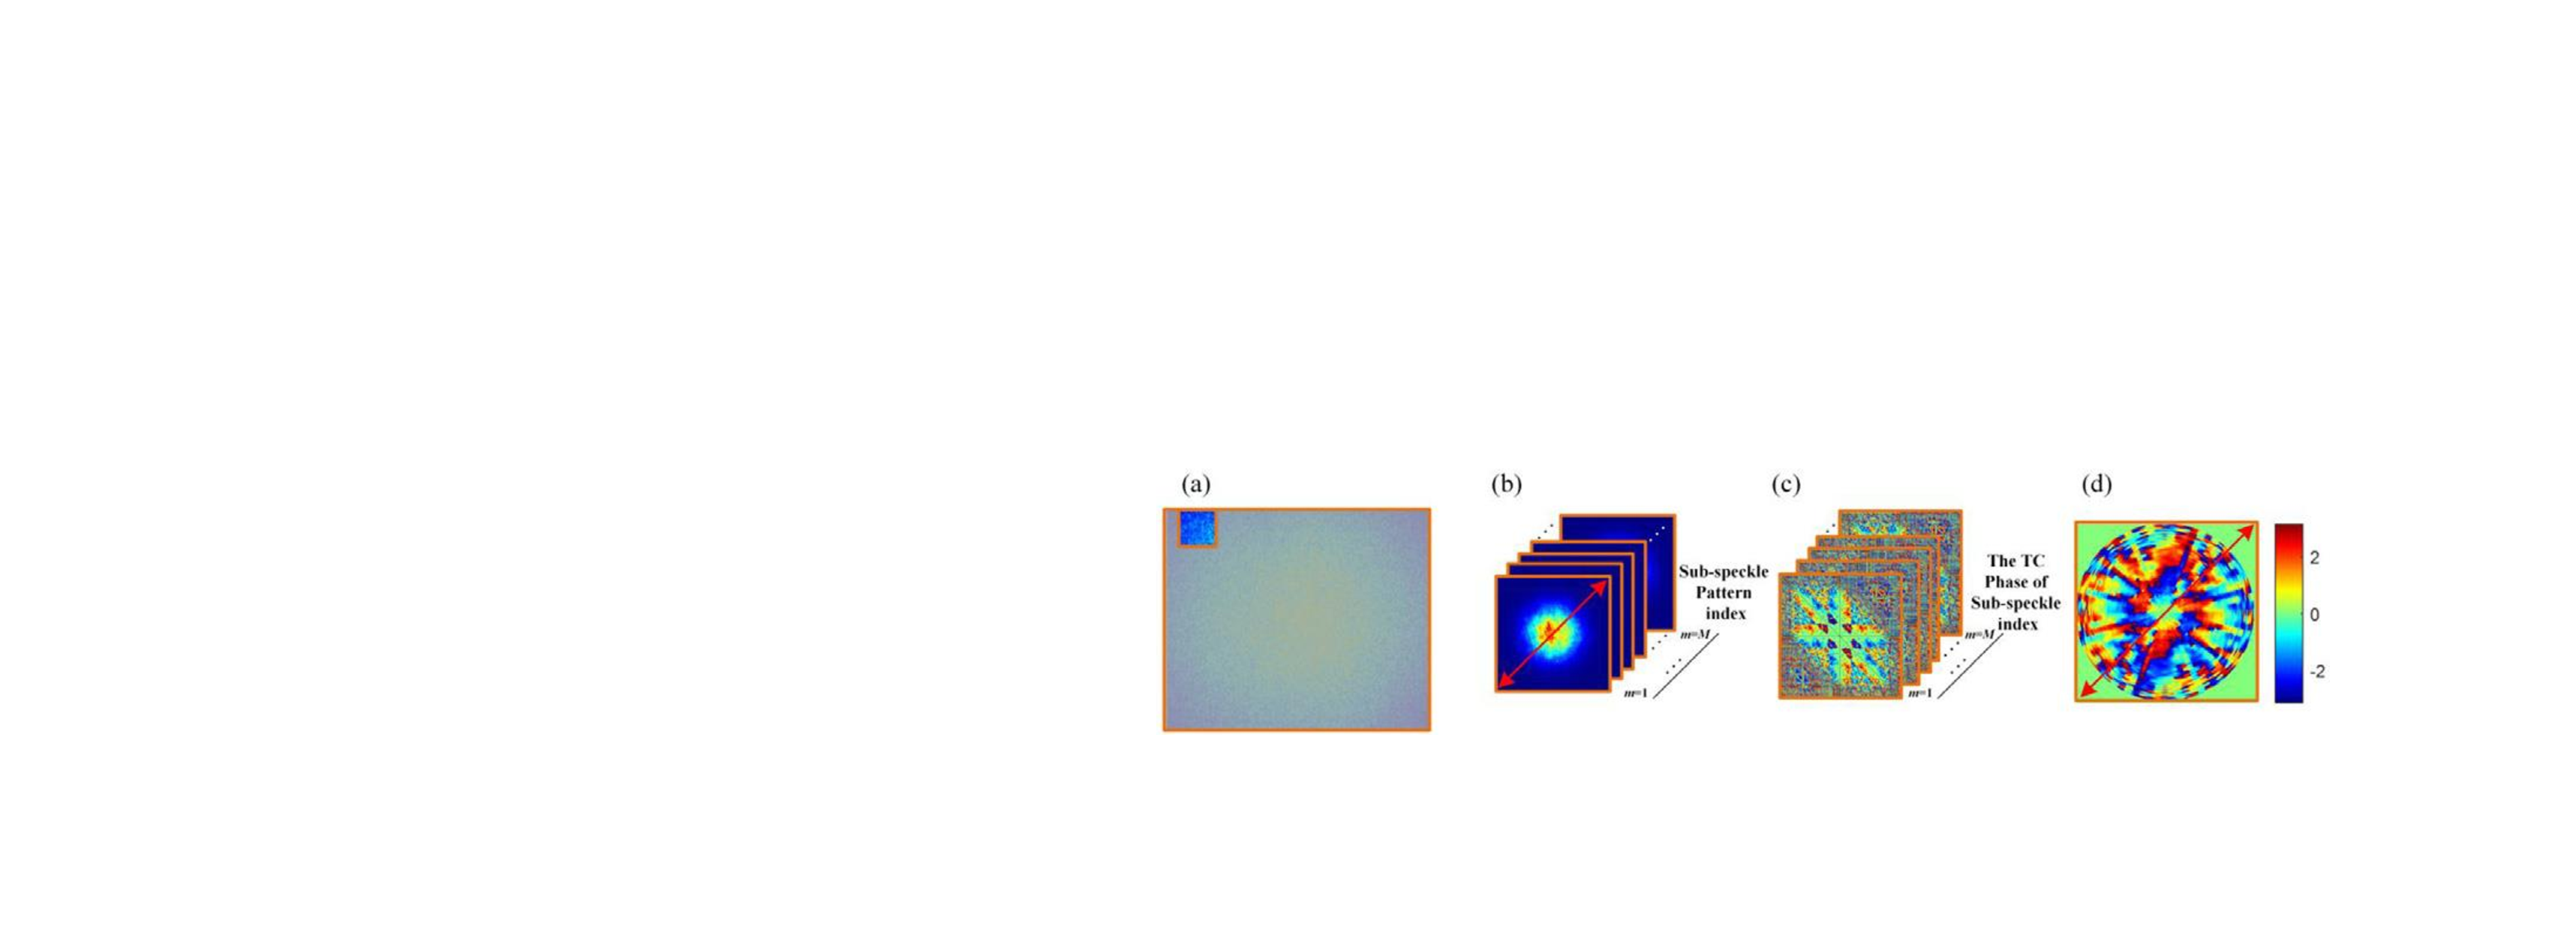
\includegraphics[scale=0.55]{C4.fig3}
	\caption{三阶相关的相位恢复算法流程如图}
	\label{fig:4.3}
\end{figure}

在此相位恢复过程中,隐藏目标的傅立叶相位将从众多子散斑图案中所恢复。首先,我们通过应用 $W_m(x,y)$的方窗函数将散斑图案(\ref{fig:4.3}a)划分为$M$个子散斑图案$I_m(x,y)$(\ref{fig:4.3}b)。其中,每个子散斑图案$I_m(x,y)$具有相同的宽度和高度,统一大小尺寸的子散斑将有助于后期的并行信号处理,且子散斑之间选取重叠区域为$90\%$。

第$m$个子散斑图案$I_m(x,y)$的强度分布可以表示为\cite{goodman_speckle_2007,goodman_introduction_2005}:

\begin{equation}
\begin{aligned}
    I_m = O*S_m
\end{aligned}
\label{eq:4.4}
\end{equation}其中,$O$表示目标的强度分布;$S_m$表示第$m$个子散斑图案所对应的PSF。

在傅里叶空间,公式(\ref{eq:4.5})可以表示为\cite{goodman_speckle_2007,goodman_introduction_2005}:
\begin{equation}
\begin{aligned}
    \mathcal{F} \{ I_m \} = C_m*\mathcal{F}\{ O \}
\end{aligned}
\label{eq:4.5}
\end{equation}其中,$C_m$表示第$m$个子散斑图案所对应系统的光学传递函数(Optical Transfer Function, OTF)。

当目标位于OME范围之内时,其成想系统可以看作是为多个点源目标的系统相应函数的非相干叠加\cite{goodman_speckle_2007,goodman_introduction_2005}。因此,该系统的振幅传递函数$H_m$可以展开为两个函数的乘积如公式(\ref{eq:4.6})所示。
\begin{equation}
\begin{aligned}
    H_m = P_m \cdot R_m
\end{aligned}
\label{eq:4.6}
\end{equation}其中,$P_m$表示散射介质所引入的影响,$R_m$表示光瞳函数所引入的影响。在此我们假设$R_m$为一个平稳的随机变量。

同时,OTF,$C_m$,是振幅传递函数$H_m$的归一化自相关,即:
\begin{equation}
\begin{aligned}
    C_m(\mu) &= \frac{\int{H_m(\mu) \cdot H_m^{*}(\mu + \mu^{\prime})}\mathrm{d}{\mu^{\prime}}}{\iint{|H_m(\mu^{\prime})|^2}\mathrm{d}{\mu^{\prime}}}\\
    &=\frac{\int{P_m(\mu) \cdot P_m^{*}(\mu + \mu^{\prime})} \cdot {R_m(\mu) \cdot R_m^{*}(\mu + \mu^{\prime})} \mathrm{d}{\mu^{\prime}}}{\iint{|P_m(\mu) \cdot P_m^{*}(\mu + \mu^{\prime})} \cdot {R_m(\mu) \cdot R_m^{*}(\mu + \mu^{\prime})}|^2 \mathrm{d}{\mu^{\prime}}}
\end{aligned}
\label{eq:4.7}
\end{equation}

根据三阶相关理论\cite{lohmann_speckle_1983,northcott_algorithms_1988},公式(\ref{eq:4.5})可以表示为:

\begin{equation}
\begin{aligned}
    \mathcal{F} \{ I_m \}^{(3)} = C_m^{(3)}*\mathcal{F}\{ O \}^{(3)}
\end{aligned}
\label{eq:4.8}
\end{equation}其中,$( \cdot ) ^{(3)}$表示三阶相关运算。

在天文成像中,可以通过多帧图像平均的方式获得光学系统的OTF。透过散射介质成像,其成像模型与天文成像中的模型极其相似。天文成像通过时间平均的方式实现了光学系统OTF的获取,我们将在散斑成像中通过空间平均的方式实现。我们将将散斑图划分为$M$个子散斑图来执行,假设每个子散斑具有各自的OTF。因此,通过散射介质成像的OTF可以表示为:
\begin{equation}
\begin{aligned}
    C(\mu) = \langle C_m(\mu)  \rangle
\end{aligned}
\label{eq:4.9}
\end{equation}其中,$\langle \cdot  \rangle$表示平均运算。

根据三阶相关理论\cite{lohmann_speckle_1983,northcott_algorithms_1988},公式(\ref{eq:4.9})可以表示为:
\begin{equation}
\begin{aligned}
    \langle C_m(\mu,\nu)^{(3)} \rangle= \langle C_m(\mu) C_m(\nu) C_m(-\mu-\nu)  \rangle
\end{aligned}
\label{eq:4.10}
\end{equation}然后,我们将公式(\ref{eq:4.7})带入公式(\ref{eq:4.10})可以获得:

\begin{equation}
\begin{aligned}
    \langle C_m(\mu,\nu)^{(3)} \rangle= &\iiint P_{m}(\mu^{\prime}) P_{m}^{*}(\mu + \mu^{\prime}) P_{m}(\mu^{\prime}) P_{m}^{*}(\mu^{\prime} + \nu) P_{m}(\omega) P_{m}^{*}(\omega -\mu - \nu) \\ &\langle R_{m}(\mu^{\prime}) R_{m}^{*}(\mu + \mu^{\prime}) R_{m}(\mu^{\prime}) R_{m}^{*}(\mu^{\prime} + \nu) R_{m}(\omega) R_{m}^{*}(\omega -\mu - \nu) \rangle \mathrm{d}{\mu^{\prime}} \mathrm{d}{\nu^{\prime}} \mathrm{d}{\omega}
\end{aligned}
\label{eq:4.11}
\end{equation}

根据散射特性,我们可知散射介质的散射效应$R_{m}$是符合高斯统计且具有各态历经性的特点,并且相互之间的相关函数为$\delta$,所以我们将天文学中的时间平均替换为空间平均,即;

\begin{equation}
\begin{aligned}
    \langle R_{m}(\mu^{\prime}) R_{m}^{*}(\mu^{\prime}+\mu) \rangle= \delta(\mu)
\end{aligned}
\label{eq:4.12}
\end{equation}

将公式(\ref{eq:4.12})带入公式(\ref{eq:4.11}),我们可以获得

\begin{equation}
\begin{aligned}
    \langle C_m(\mu,\nu)^{(3)} \rangle = &\langle C_m(\mu) \rangle \langle C_m(\nu) \cdot C_m(-\nu-\mu) \rangle + \\
		& \langle C_m(\mu)\cdot C_m(\nu) \rangle \langle C_m(-\nu-\mu) \rangle +\\
		& \langle C_m(\nu) \rangle \langle C_m(\mu) \cdot C_m(-\nu-\mu) \rangle -\\
		& 2\langle C_m(\nu) \rangle \langle C_m(\mu)\rangle \langle C_m(-\nu-\mu) \rangle +\\
		& + \kappa(\mu,\nu)^{(3)}
\end{aligned}
\label{eq:4.13}
\end{equation}其中,函数$\kappa(\mu,\nu)^{(3)}$的定义为:

\begin{equation}
\begin{aligned}
    \kappa(\mu,\nu)^{(3)} = &\int |P_m(\omega)|^2 \cdot |P_m(\mu+\nu+\omega)|^2 \\
		& \left[|P_m(\mu + \omega)|^2 + |P_m(\nu+\omega)|^2 \right]^2 \mathrm{d}{\omega}
\end{aligned}
\label{eq:4.14}
\end{equation}

由公式(\ref{eq:4.1})可知,$\kappa(\mu,\nu)^{(3)}$取决于散射介质孔径函数的影响$P_m$。然后,我们将公式(\ref{eq:4.13})带入公式(\ref{eq:4.8})可得:

\begin{equation}
\begin{aligned}
    \langle C_m(\mu,\nu)^{(3)} \rangle \cdot \mathcal{F}\{ O \}^{(3)}= &\langle C_m(\mu) \rangle \langle C_m(\nu) \cdot C_m(-\nu-\mu) \rangle \cdot \mathcal{F}\{ O \}^{(3)}+ \\
		& \langle C_m(\mu)\cdot C_m(\nu) \rangle \langle C_m(-\nu-\mu) \rangle \cdot \mathcal{F}\{ O \}^{(3)}+\\
		& \langle C_m(\nu) \rangle \langle C_m(\mu) \cdot C_m(-\nu-\mu) \rangle \cdot \mathcal{F}\{ O \}^{(3)}-\\
		& 2\langle C_m(\nu) \rangle \langle C_m(\mu)\rangle \langle C_m(-\nu-\mu) \rangle \cdot \mathcal{F}\{ O \}^{(3)}+\\
		& + \kappa(\mu,\nu)^{(3)}\cdot \mathcal{F}\{ O \}^{(3)}
\end{aligned}
\label{eq:4.15}
\end{equation}
在公式(\ref{eq:4.15})中,$\langle C_m(\mu) \rangle$拥有与天文散斑成像中长曝光时OTF相同的特性。因此,他是非零的,只有轴上$\mu = 0$,$\nu = 0$,$\mu = -\nu$和$\mu =\nu= 0$时值为零。所以,继续推导公式(\ref{eq:4.15})可得:

\begin{equation}
\begin{aligned}
    \langle C_m(\mu,\nu)^{(3)} \rangle \cdot \mathcal{F}\{ O \}^{(3)} \approx \kappa(\mu,\nu)^{(3)}\cdot \mathcal{F}\{ O \}^{(3)} \approx   \langle \mathcal{F}\{ I_m \}^{(3)} \rangle
\end{aligned}
\label{eq:4.16}
\end{equation}

根据公式(\ref{eq:4.14})可知:$\kappa(\mu,\nu)^{(3)}$与散射介质的影响$R_m$无关。因此,公式(\ref{eq:4.16})可以简化为:

\begin{equation}
\begin{aligned}
   \mathcal{F}\{ O \}^{(3)} \approx   \langle \mathcal{F}\{ I_m \}^{(3)} \rangle
\end{aligned}
\label{eq:4.17}
\end{equation}

因此,目标的三阶相关相位$\mathcal{F}\{ O \}^{(3)}$近似等于所有子散斑三阶相关相位的平均$\langle \mathcal{F}\{ I_m \}^{(3)} \rangle$。

根据三阶相关理论,目标的傅里叶相位$\phi_{l}$和子散斑图案的三阶相关的相位$\beta_{m}^{(3)}$应满足方程:

\begin{equation}
\begin{aligned}
   \mbox{exp}[i\phi(l)]= \mbox{exp}\left[i(\phi(\mu)+\phi(\nu)- \langle {\beta_{m}^{(3)}(\mu,\nu)} \rangle)\right]
\end{aligned}
\label{eq:4.18}
\end{equation}其中,$\nu=l-\mu$,
\begin{equation}
\begin{aligned}
  {\beta_{m}^{(3)}(\mu,\nu)}= \mbox{arg}\left[\mathcal{F}\{I_m\}(\mu)\cdot \mathcal{F}\{I_m\}(\nu) \cdot \mathcal{F}\{I_m\}(-\mu-\nu)\right]
\end{aligned}
\label{eq:4.19}
\end{equation}
然后,根据公式(\ref{eq:4.18})可以恢复隐藏目标的傅里叶相位信息。在傅立叶域中,第一个频率的值与物体的位置有关。在实践中,我们将第一个频率$\phi_{1}$ 和$\phi_{0}$的相位设置为零。为了避免直接计算二维图像的三阶相关所引入的巨大计算工作,通过Radon变换\cite{ayers_knoxthompson_1988}将子散斑图案转换为多个一维信号,计算多个以为信号的三阶相关。如图\ref{fig:4.3}c所示,其为来自第$m$个子散斑的某一以维信号的三阶相位${\beta_{m}^{(3)}(\mu,\nu)}$,在此过程中,使用“Higher Order
Spectral Analysis Toolbox”Matlab工具包进行三阶相关的相位计算。我们根据中心切片定理,将多个角度的Radon变化后所最终获取的一位信号的傅里叶相位信息进行整合,获得最终的傅里叶相位信息。

\subsection{仿真验证及方法对比}

\begin{figure}[htp]
	\centering
	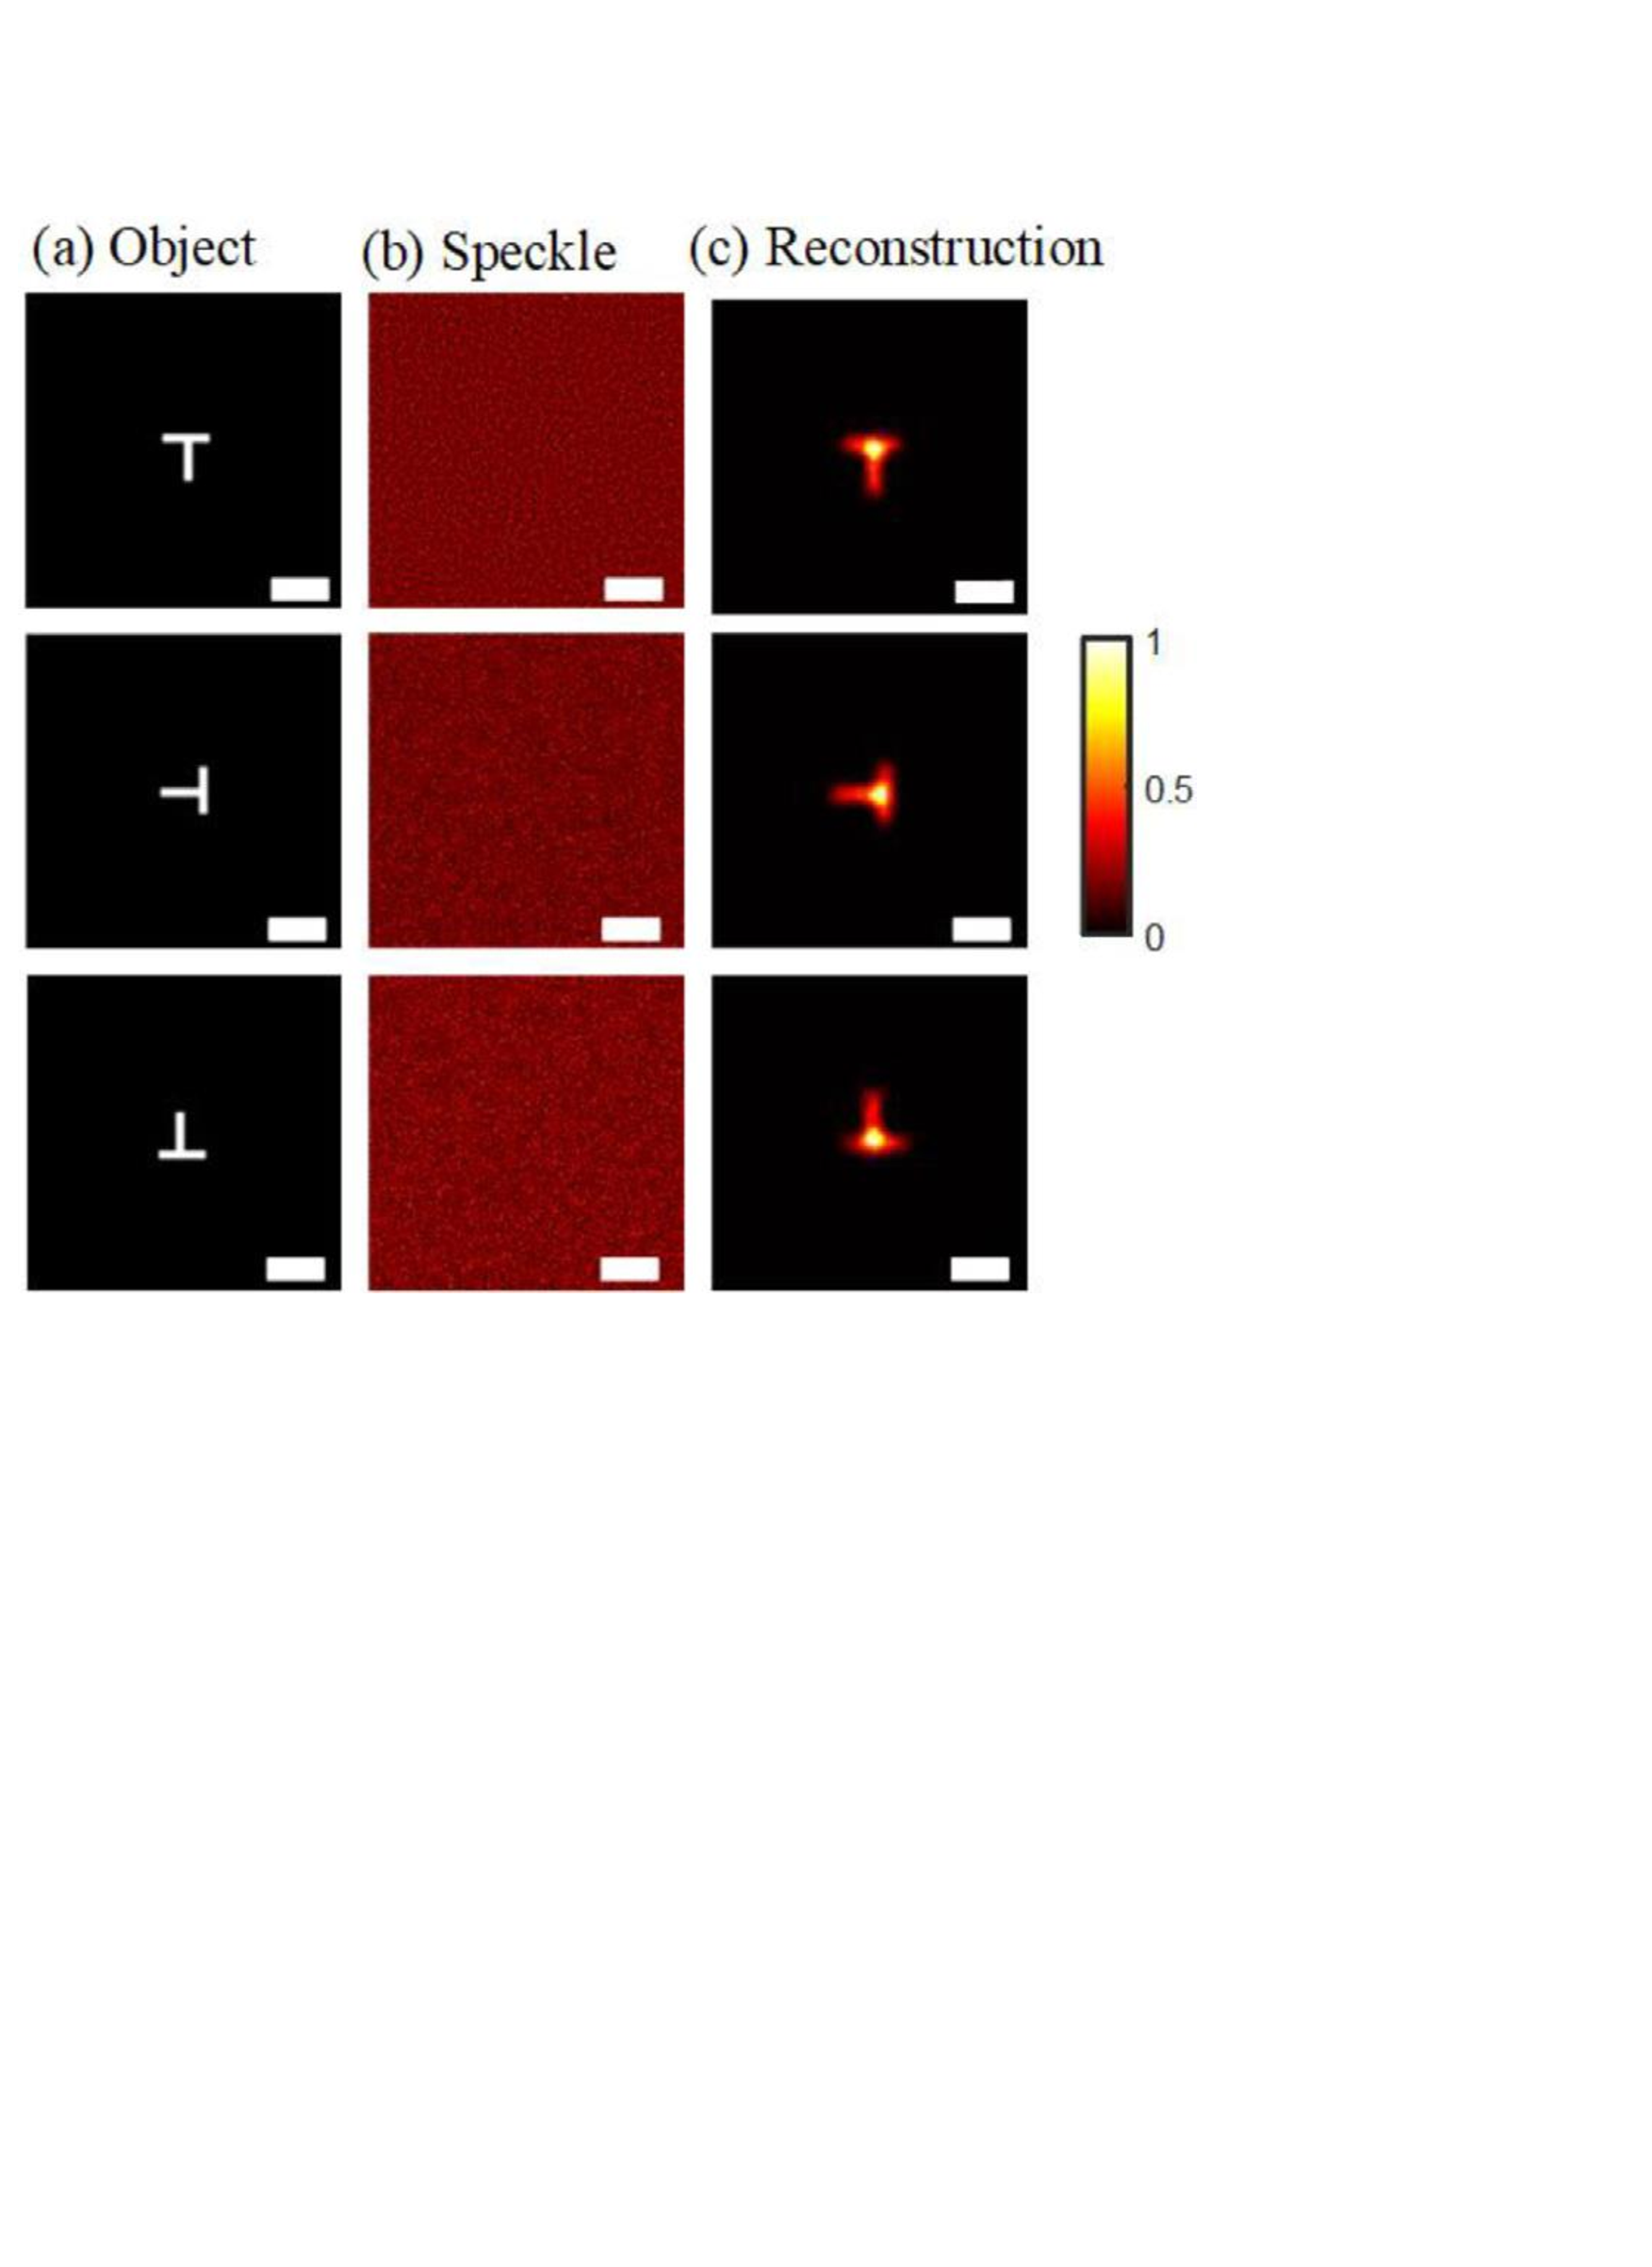
\includegraphics[scale=0.40]{C4.fig4}
	\caption{基于三阶相关相位恢复的散斑成像仿真结果}
	\label{fig:4.4}
\end{figure}

为了验证基于三阶相关相位恢复的散斑成像的有效性,我们进行了相应的数字模拟仿真,其结果如图\ref{fig:4.4}所示。从图\ref{fig:4.4}可以看出,原始目标的方向与重建的目标的方向完全保持一致,该特性保证了透过散射介质彩色成像的顺利进行。此外,我们将不同的相位恢复算法:三阶相关,HIO和广义近似信息传递的相位恢复算法(Phase Retrieval via Generalized Approximate Message Passing,prGAMP)所重建的结果进行了对比,其结果如图\ref{fig:4.5}所示,其中图(a)为原始目标;(b)为散斑图案;(c)为三阶相关相位恢复算法所对应的重建结果;(d)为HIO算法所对应的重建结果;(e)为 prGAMP算法所对应的重建结果。实验结果同时也证明了基于三阶相位恢复算法能够保证正确的恢复隐藏目标的图像。通过以上的仿真结果和实验结果可以得出:三阶相位相关相位恢复算法能够有效的恢复隐藏目标的方向信息。于是,这一特性能够确保在彩色成像中不用颜色通道中的方向时正确的,该特性有利于合成彩色图像。

\begin{figure}[htp]
	\centering
	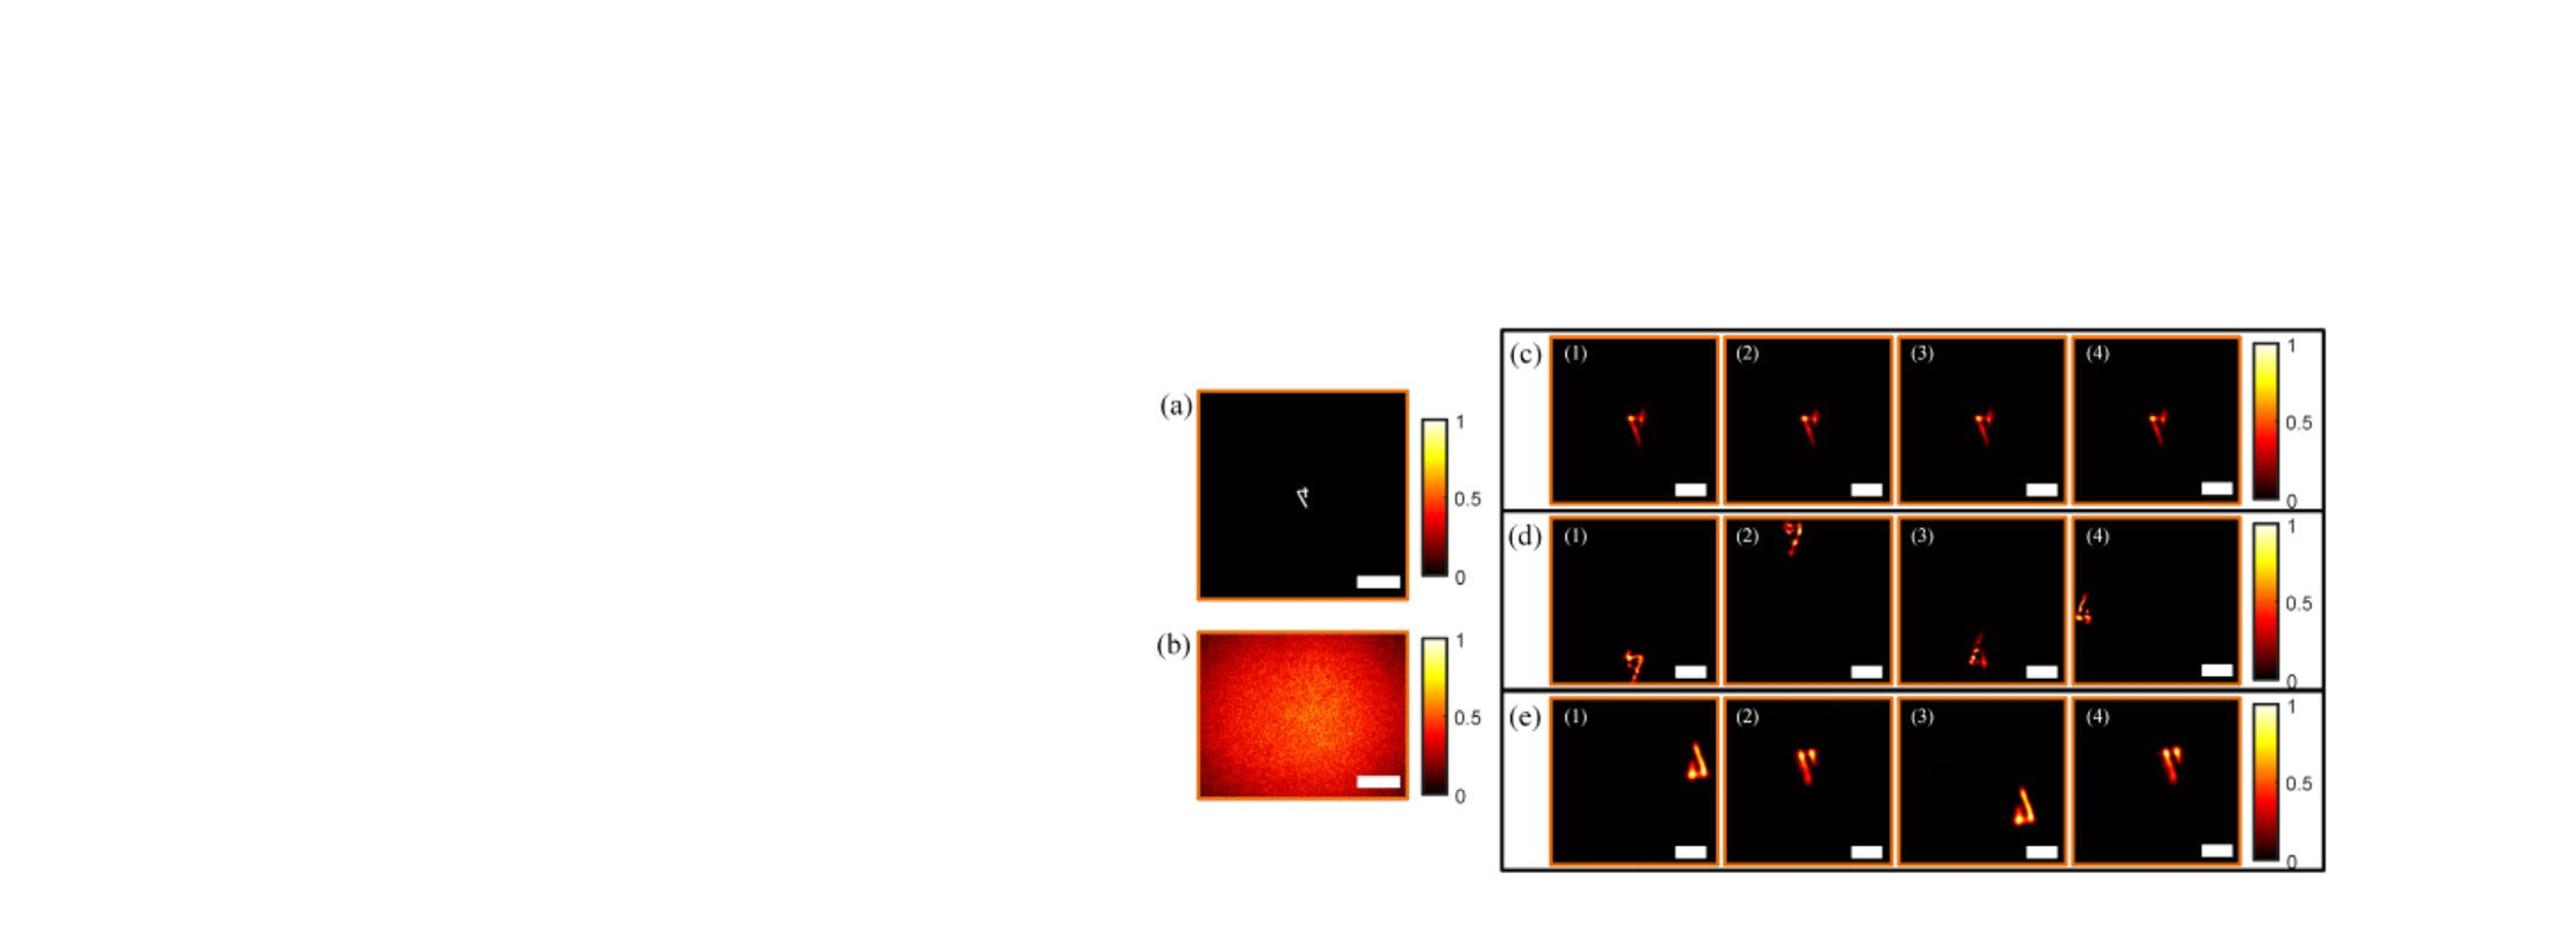
\includegraphics[scale=0.55]{C4.fig5}
	\caption{不同相位恢复算法重建结果对比}
	\label{fig:4.5}
\end{figure}

\section{成像系统与结果分析}
\subsection{成像系统}

如第2.1节所描述,隐藏目标的三阶傅里叶相位与子散斑的三阶相关傅里叶相位的平均值相等。在进行彩色成像实验之前,我们将进行再一次实验验证,确保该算法能够有效的恢复目标的方向信息。于是,我们改变目标的方向,其分别为:$0^{\circ}$,$90^{\circ}$,$180^{\circ}$和$270^{\circ}$,实验结果如图\ref{fig:4.7}所示。对于实验中的每种情况,该方法都可以有效的重建图像,并且重建图像的方向信息与原始目标的的方向信息一致。实验结果进一步表明,利用三阶相关相位恢复技术可以确保保持目标的方向信息并恢复目标的图像。

\begin{figure}[htp]
	\centering
	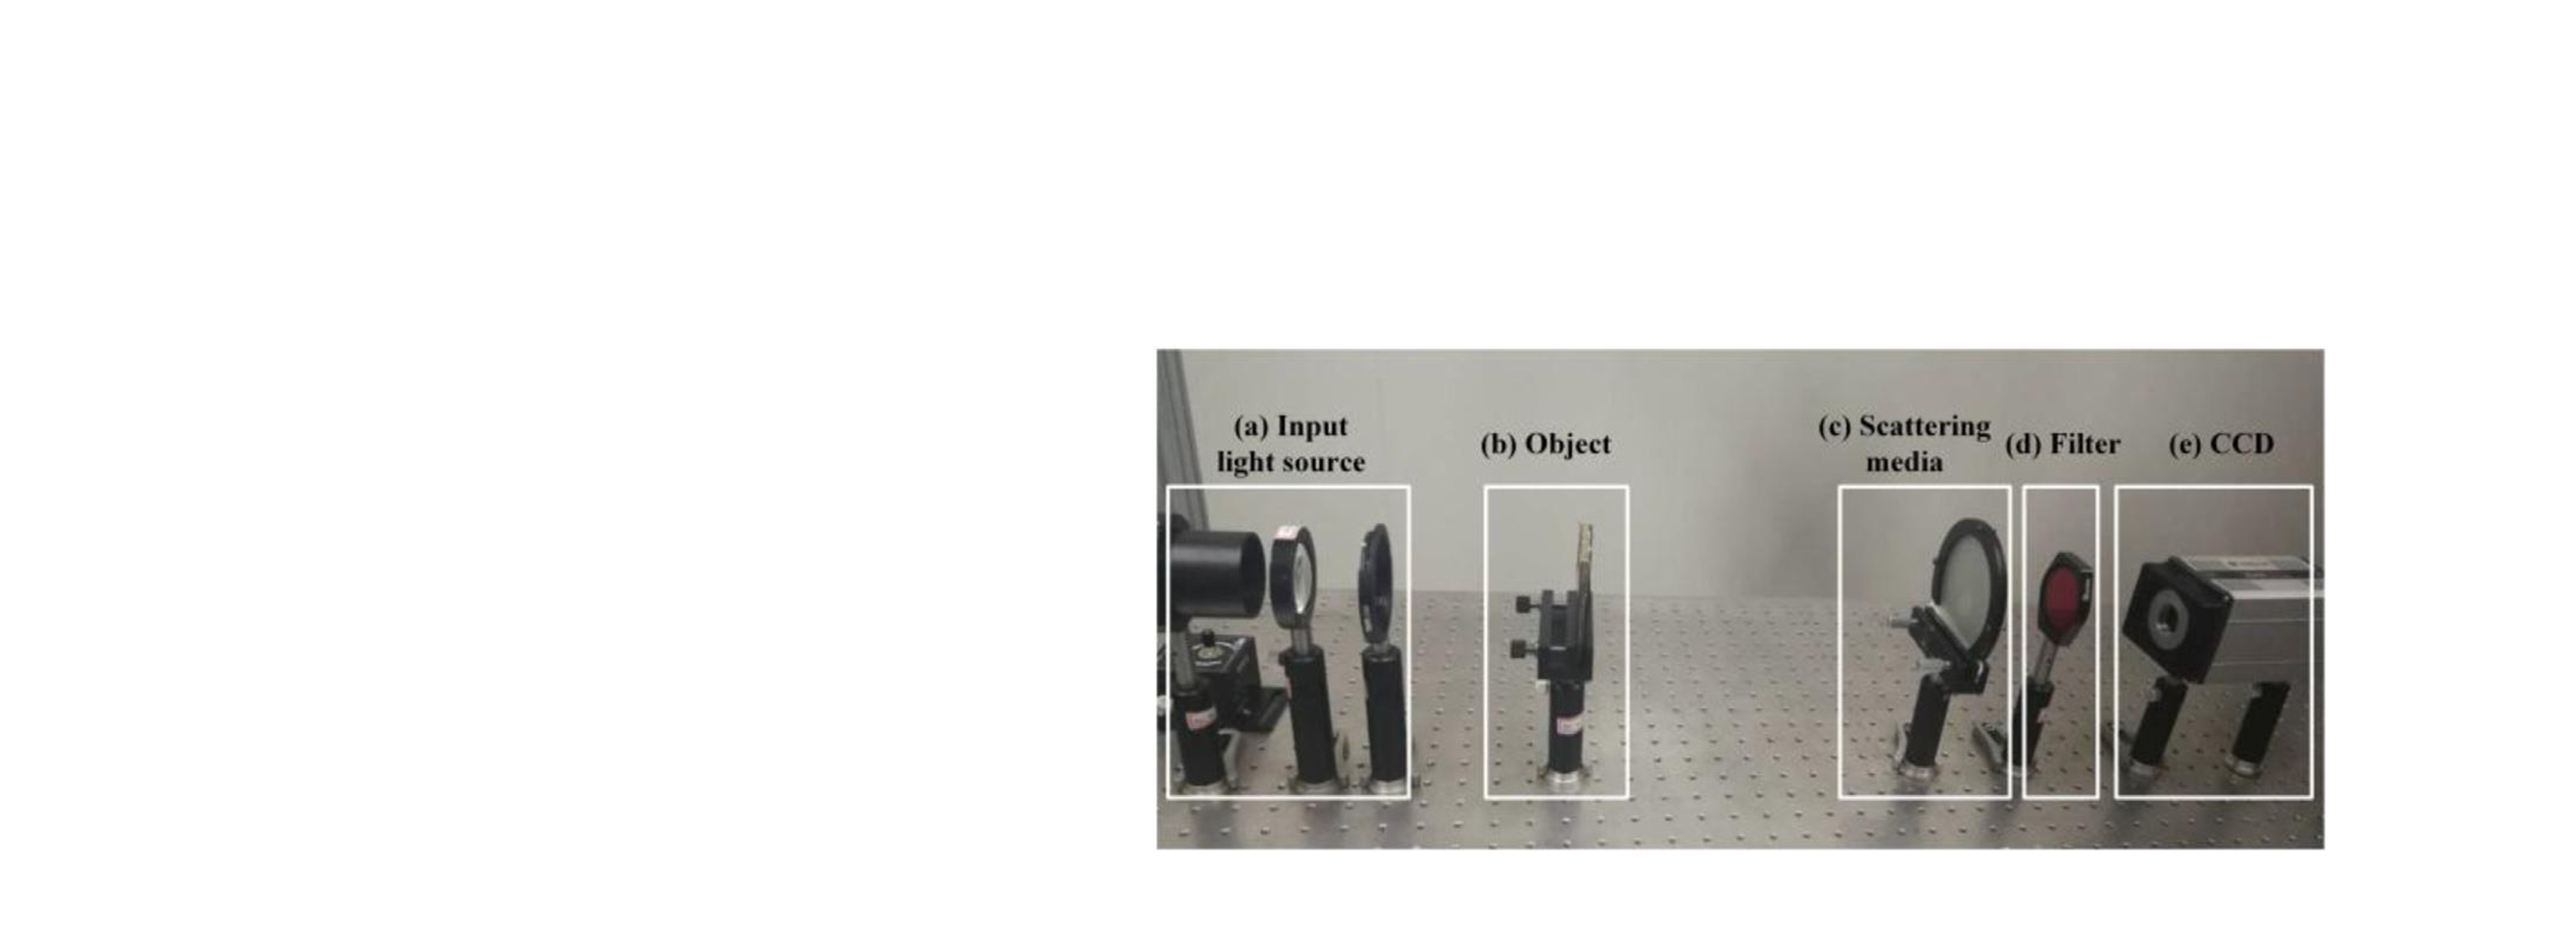
\includegraphics[scale=0.55]{C4.fig6}
	\caption{基于三阶相关相位恢复的实验装置图}
	\label{fig:4.6}
\end{figure}
\begin{figure}[htp]
	\centering
	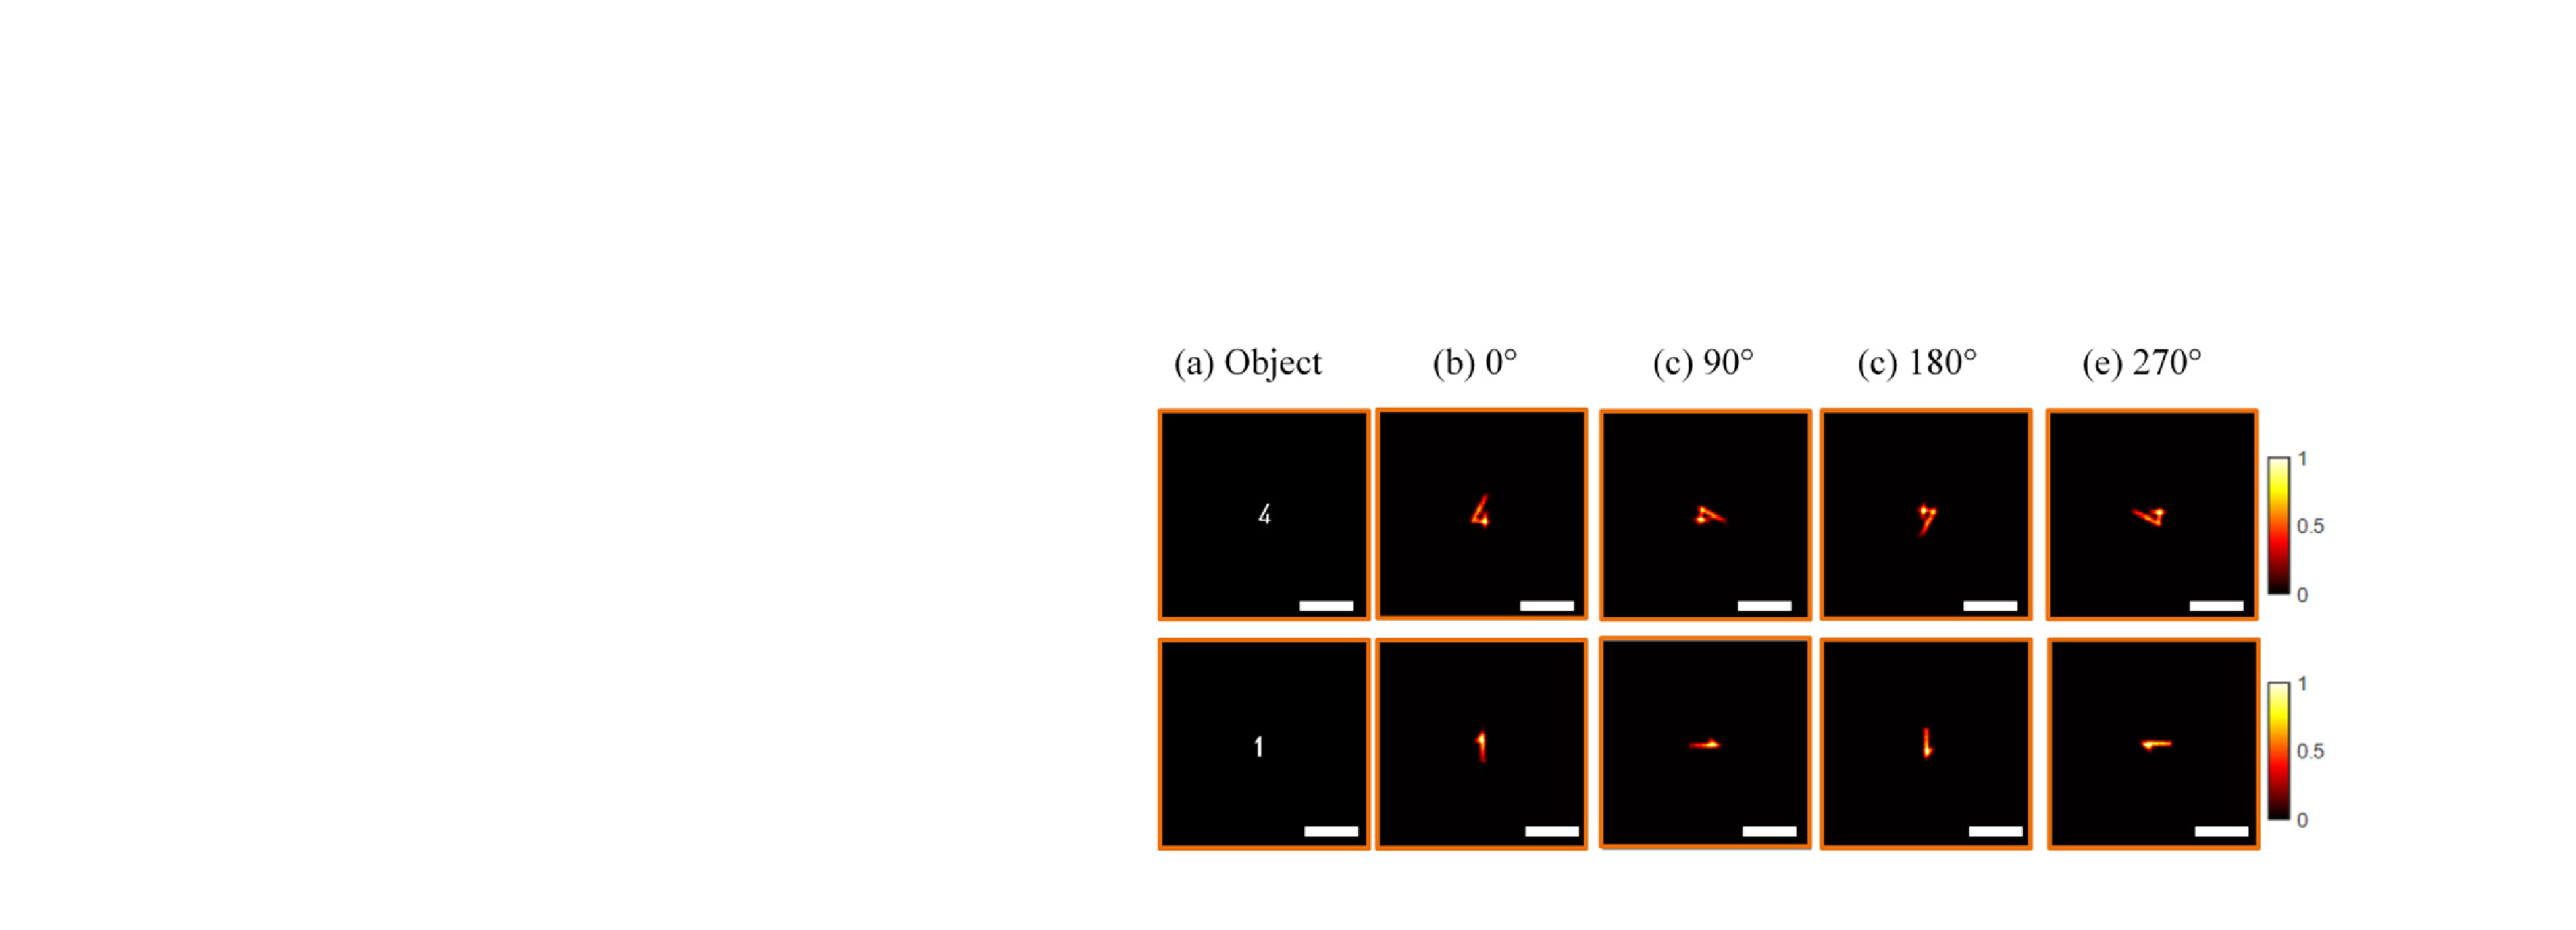
\includegraphics[scale=0.55]{C4.fig7}
	\caption{基于三阶相关相位恢复的实验结果}
	\label{fig:4.7}
\end{figure}

\subsection{实验结果}

我们采用的实验装置图如\ref{fig:4.6}所示,通过彩色打印的方式制作不同的目标。散射介质与目标的之间的距离大于为$70cm$,散射介质与相机之间的距离为$10cm$。首先,我们制作了透明的目标,验证彩色成像方法,实验结果如图\ref{fig:4.8}所示。图\ref{fig:4.8}(a)为原始目标,图\ref{fig:4.8}(b),(c)和(d)分别为利用不同干涉滤光片后所获取的不同RGB彩色通道的散斑,图\ref{fig:4.8}(e),(f)和(g)分别对应于散斑(b),(c)和(d)所重建的各自图案,图\ref{fig:4.8}(h)为通过将RGB散彩色通道进行合成的图像。当彩色成像方法被证明后,我们采用了不同的彩色目标进行了实验,实验结果如图\ref{fig:4.9}所示。

\begin{figure}[htp]
	\centering
	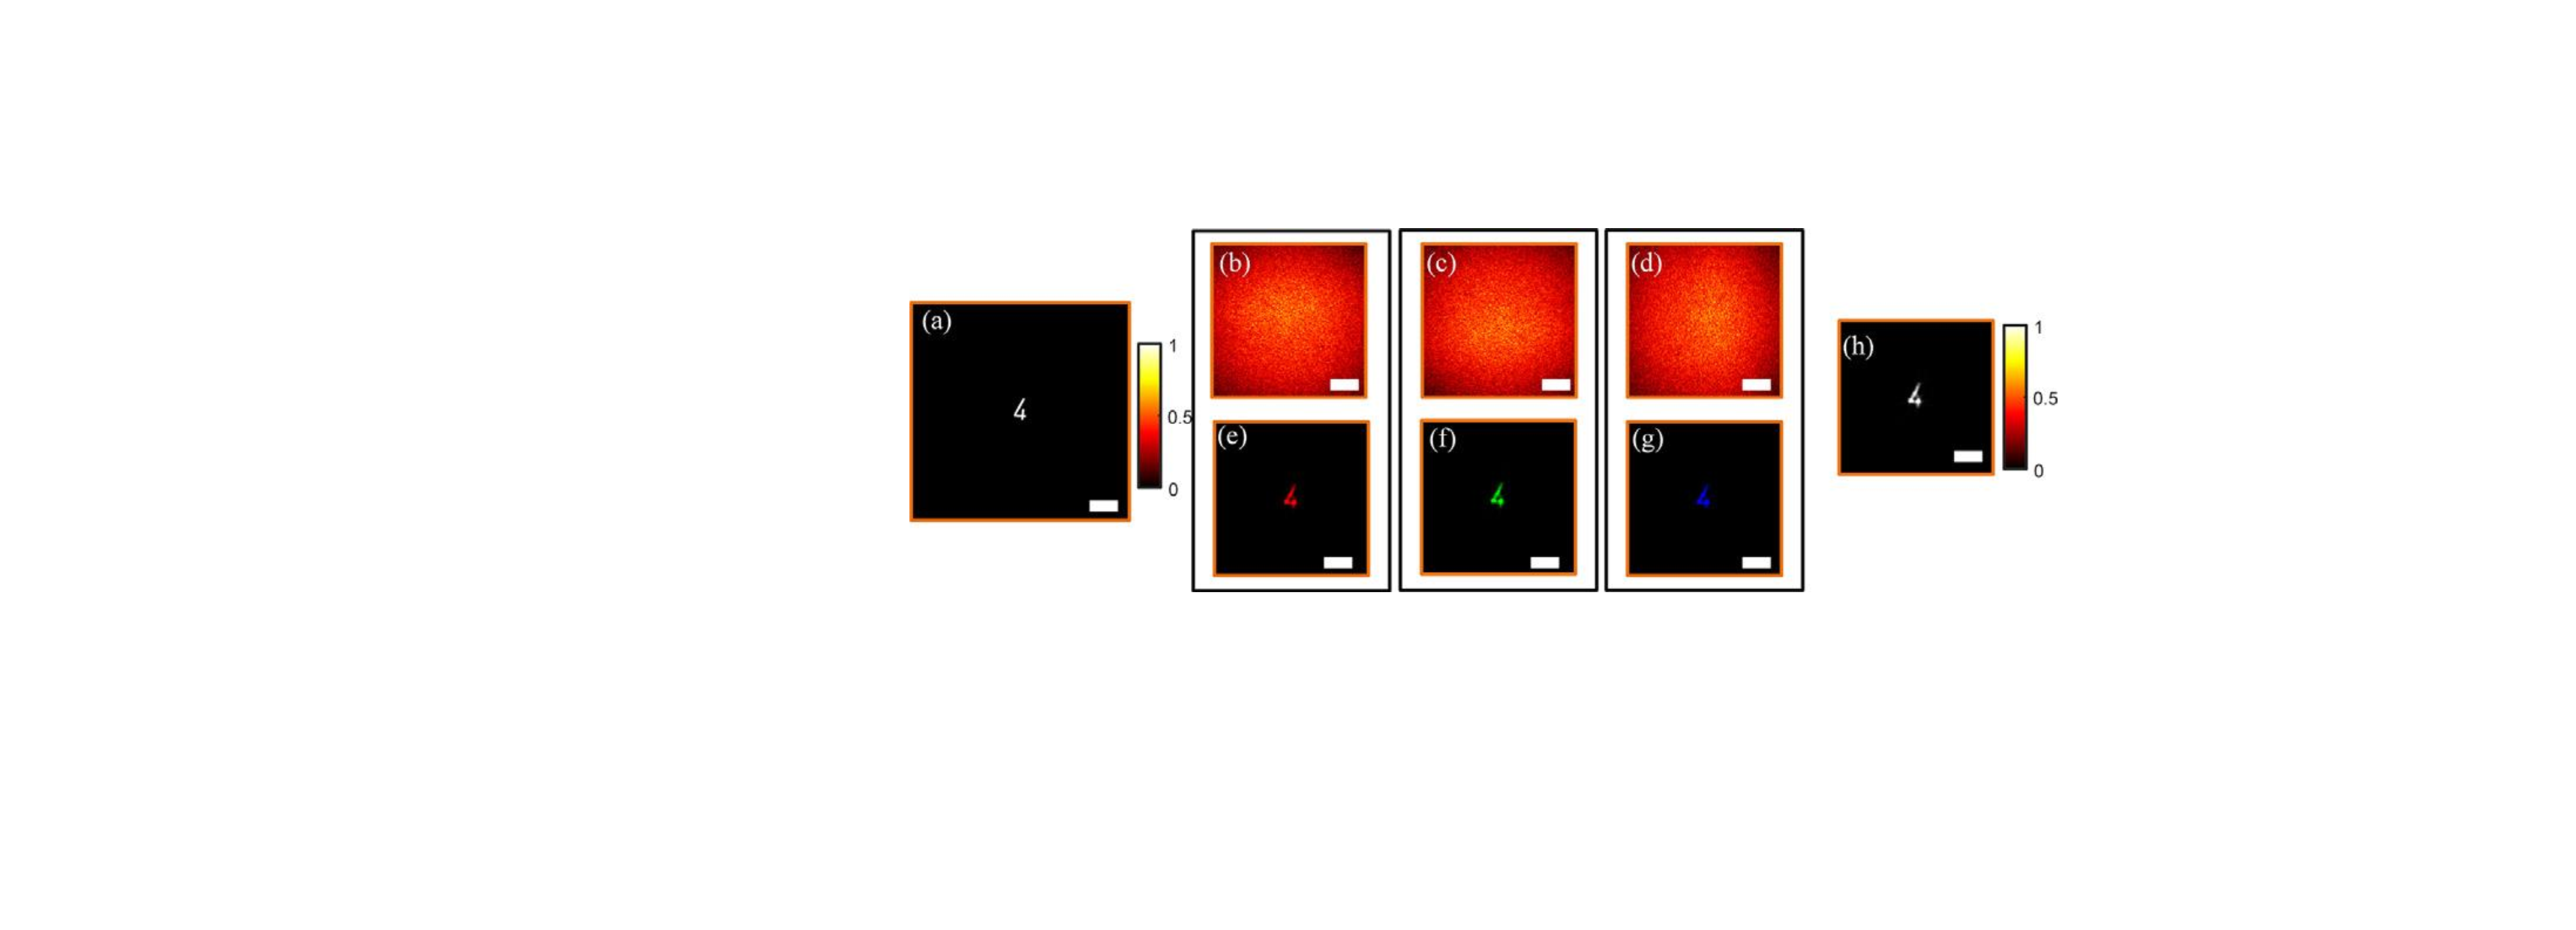
\includegraphics[scale=0.55]{C4.fig8}
	\caption{彩色实验结果}
	\label{fig:4.8}
\end{figure}
\begin{figure}[htp]
	\centering
	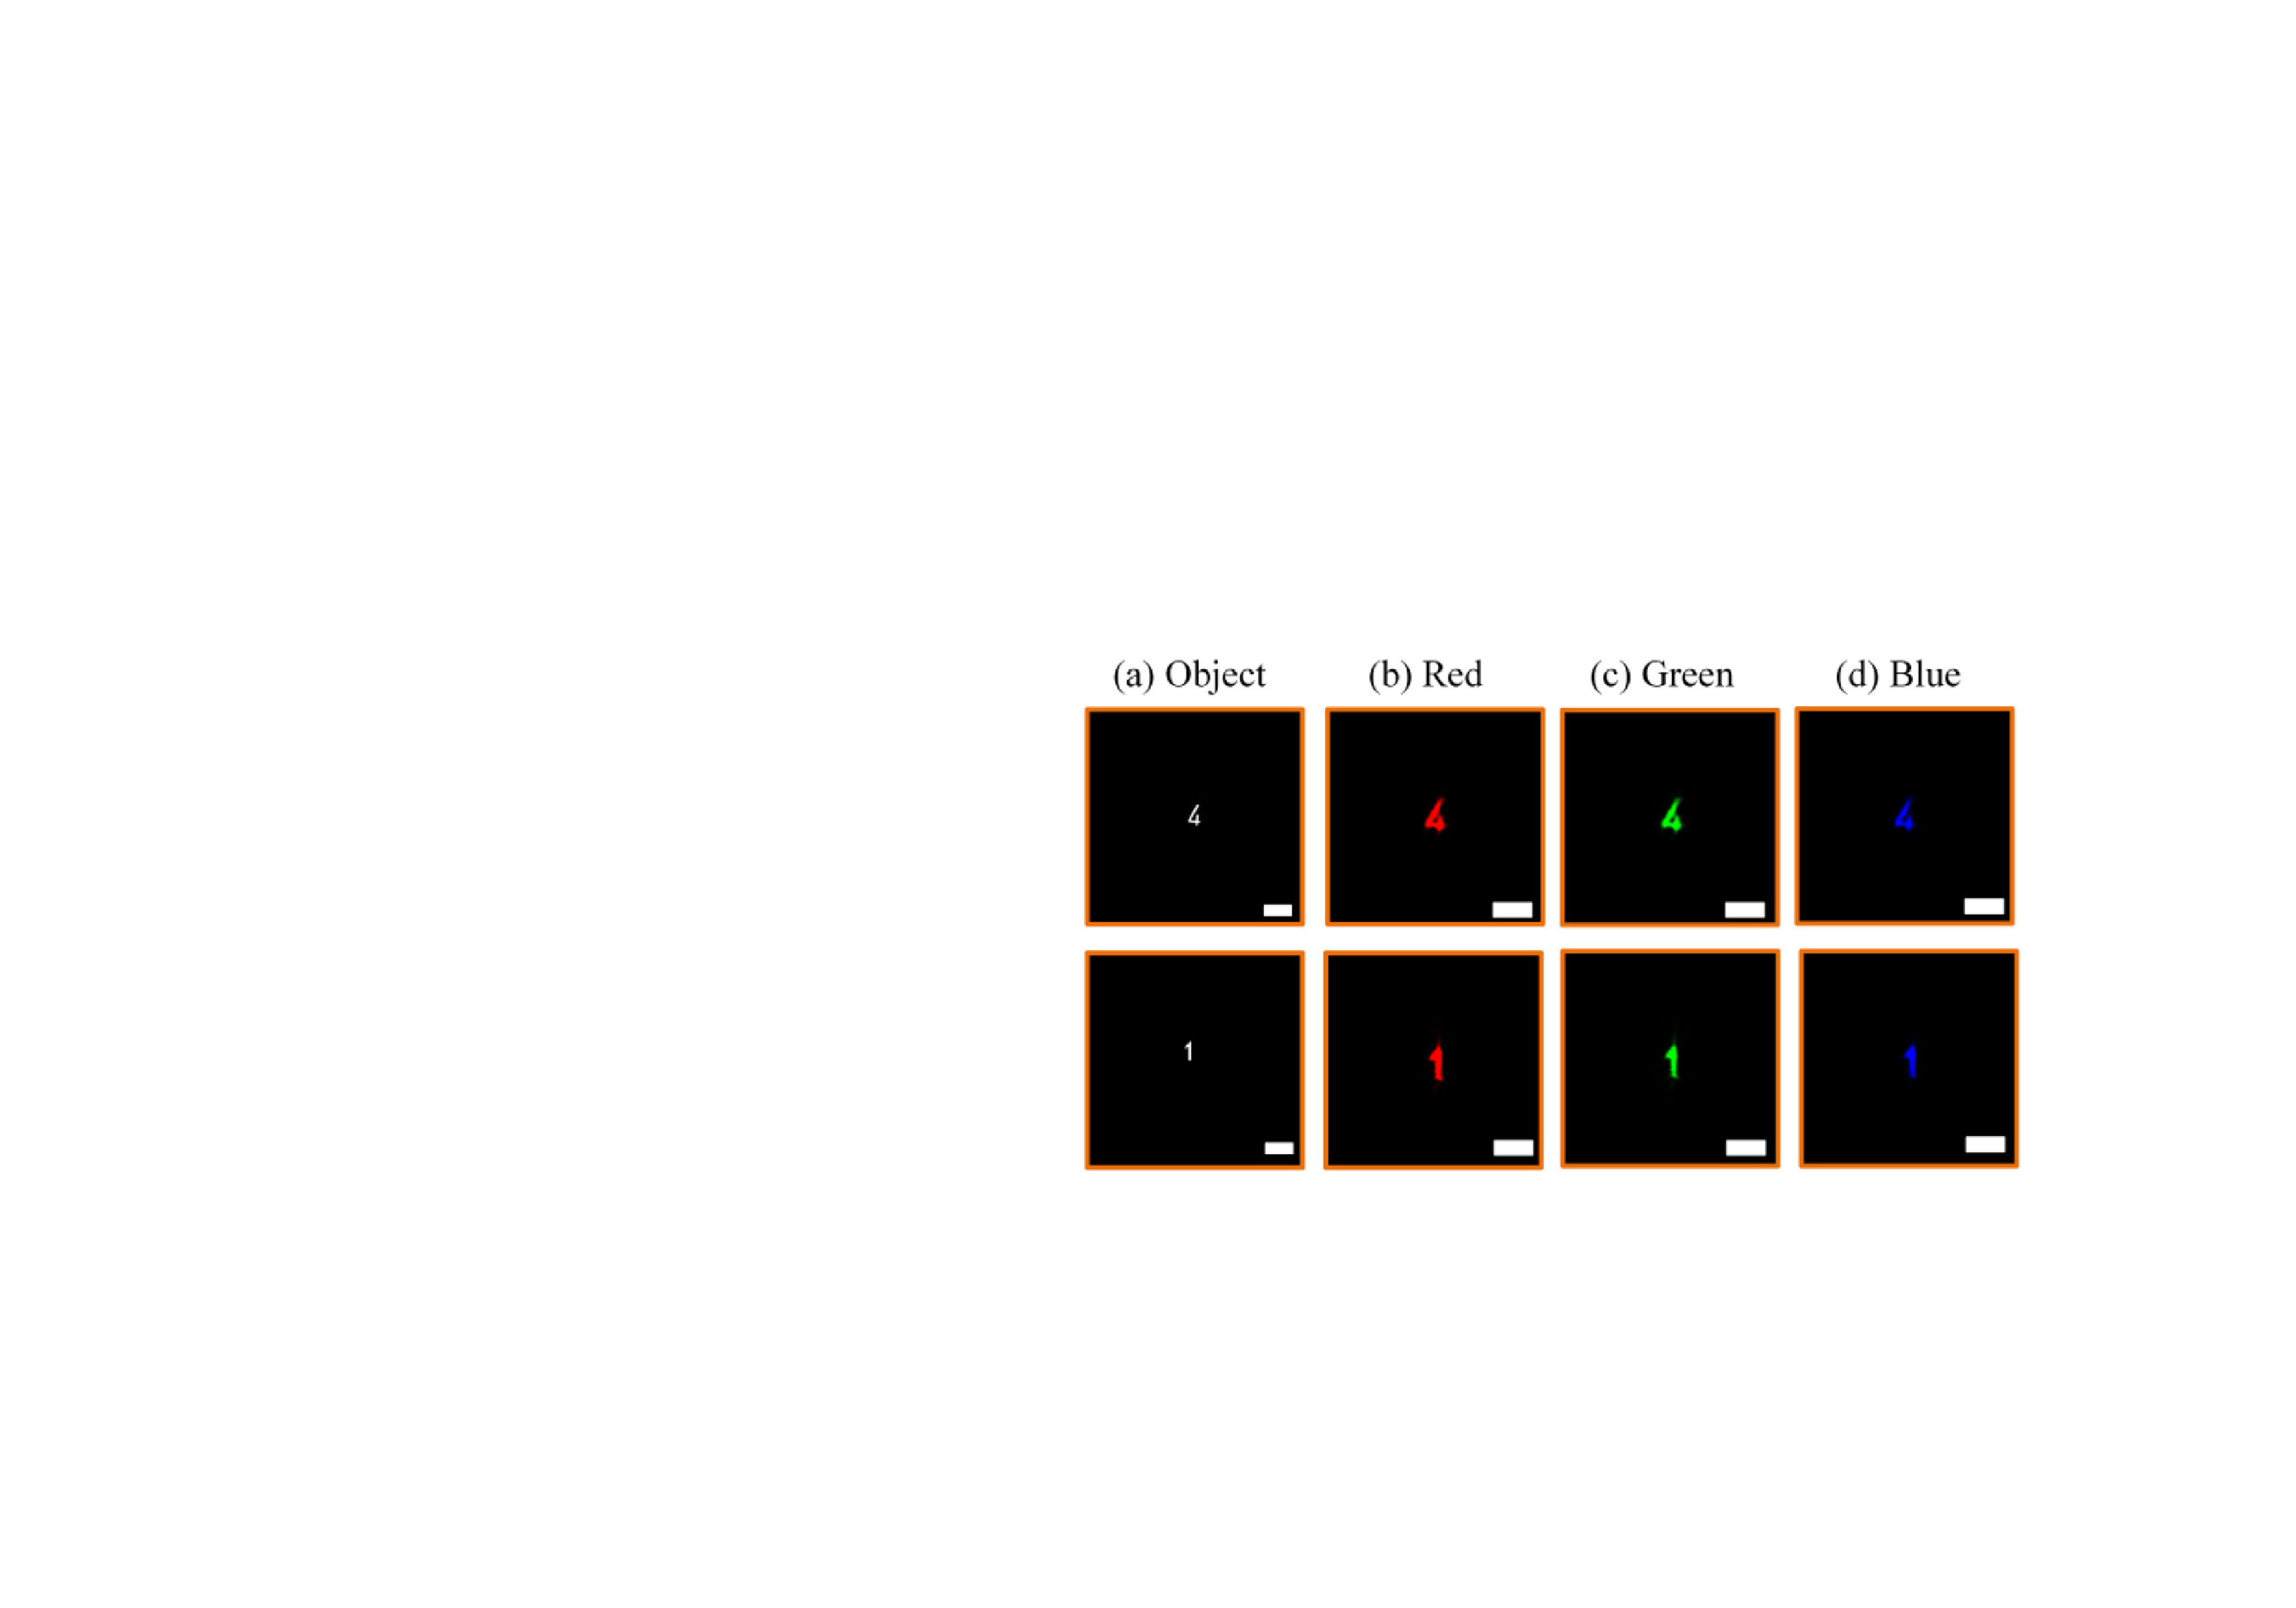
\includegraphics[scale=0.55]{C4.fig9}
	\caption{不同目标的彩色实验结果}
	\label{fig:4.9}
\end{figure}

图\ref{fig:4.8}和图\ref{fig:4.9}证明了我们所提出的透过散射介质的彩色成像方法。值得注意的是:在图\ref{fig:4.8}和图\ref{fig:4.9}中我们所使用的目标均为简单目标,即同一目标的彩色信息相同。但是在实际应用过程中,除非我们考虑复杂颜色的对象,否则证明其有效性是不够的。对于复杂的颜色对象,尽管可以通过我们所提出的通向恢复方法恢复不同颜色通道中的图案,但对象在不同颜色通道中的相对位置仍然未知。为了确定物体在不同颜色通道中的相对位置,我们采用参考目标,参考物体在不同颜色通道中的透射率几乎相等,且具有固定形状,利用参考目标去获取不同颜色通道中所恢复目标的相对位置。

为了证明我们的方法能够实现复杂彩色目标成像,我们制作了特殊的彩色目,该目标同拥有不同的三种颜色,是实验结果如图\ref{fig:4.10}所示。如图\ref{fig:4.10}(a)所示,数字“1”为绿色,数字“4”为红色,参考目标为透明目标。 图\ref{fig:4.10}(b)上部分展示了通过图像恢复方法从相应颜色通道的散斑图案中恢复的彩色图像。红色通道图像中出现数字“1”,绿色通道图像中出现数字“4”,参考对象同时出现在红色通道、绿色通道和蓝色通道中。 在图\ref{fig:4.10}(b)下部分中显示了重建图像中虚线所应的强度信息。然后根据参考目标的位置,我们将RGB通道的彩色图像进行叠加,得到图\ref{fig:4.10}(c)中的“全彩”图像。

\begin{figure}[htp]
	\centering
	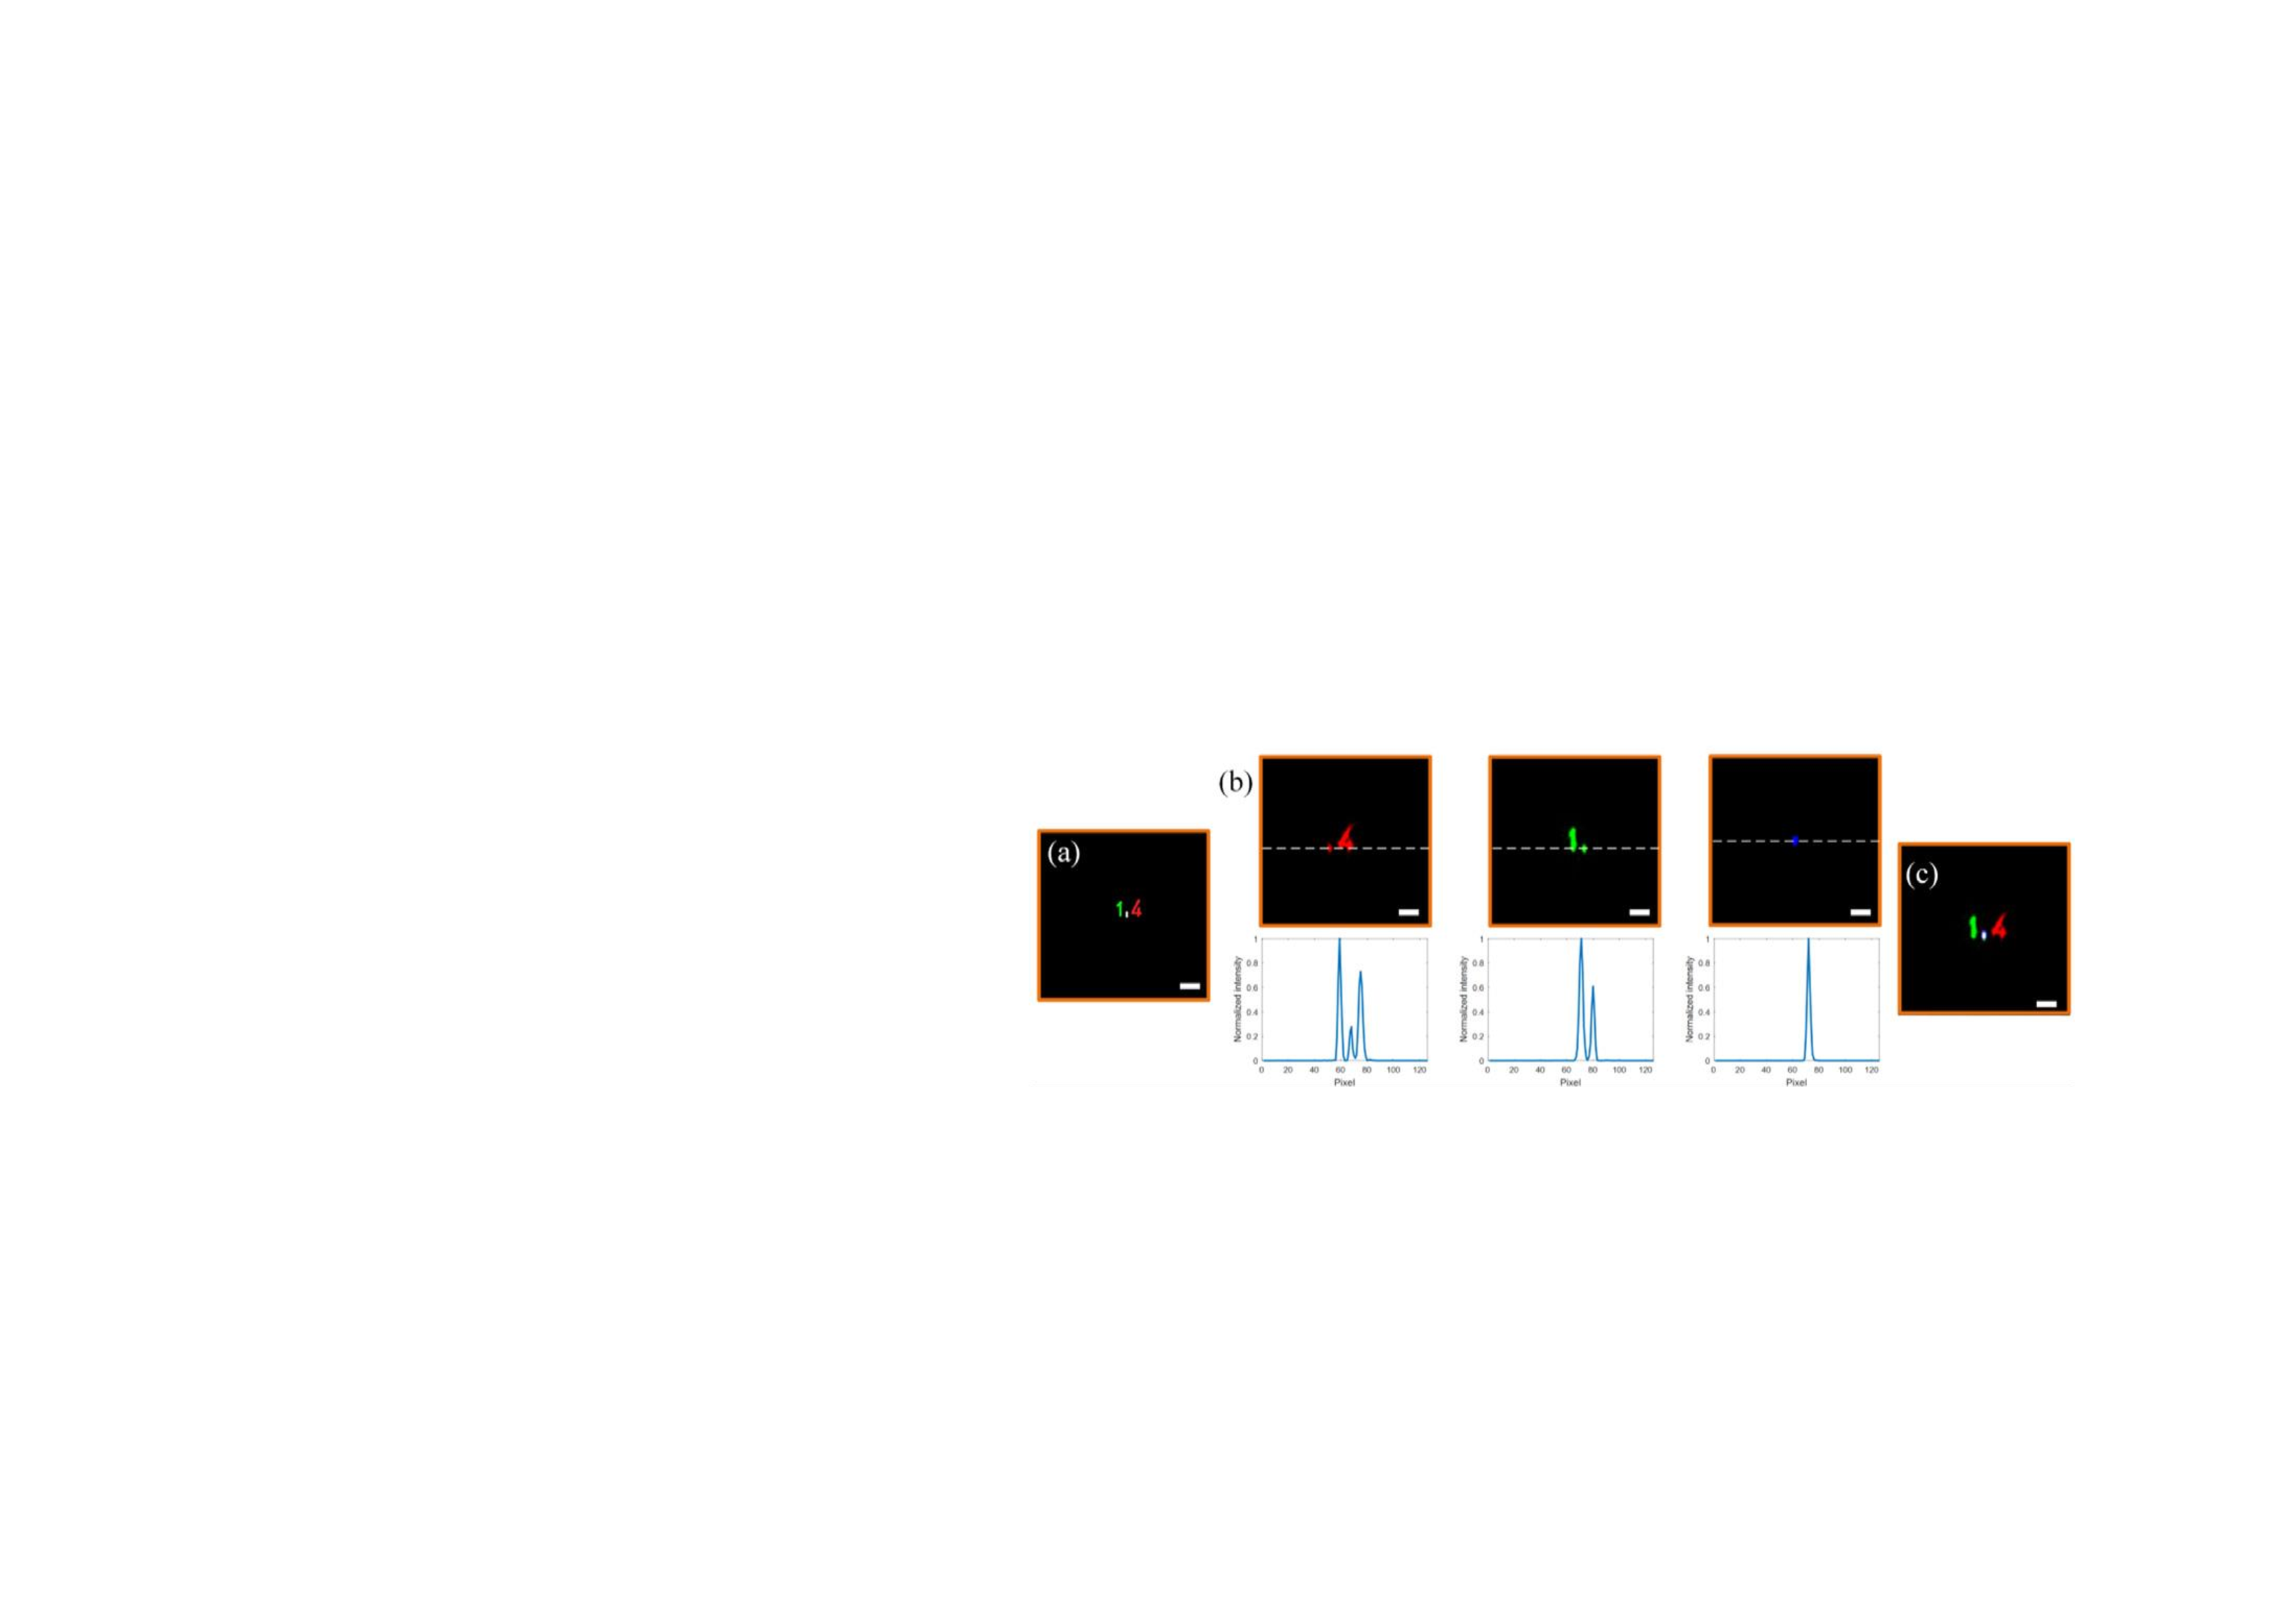
\includegraphics[scale=0.50]{C4.fig10}
	\caption{复杂目标的彩色实验结果}
	\label{fig:4.10}
\end{figure}

尽管已经提出了许多基于散斑的成像方法,但是通过散射介质进行光谱成像仍然是一项艰难的挑战。但是,我们所提出的彩色成像方法能够与传统的光谱成像方法相结合,实现光谱成像。原则上,我们用不同的干涉滤光片获取不同光谱通道的散斑,进行分别重建,然后进行数据整合。于此,我们进行了简单的实验验证,实验结果如图\ref{fig:4.11}所示。在实验中,我们获取的光谱通道分别为:$\lambda_1 =445nm$,$\lambda_2  =530nm$和$\lambda_3  =630nm$的光谱数据,分别进行图像重建显示。

\begin{figure}[htp]
	\centering
	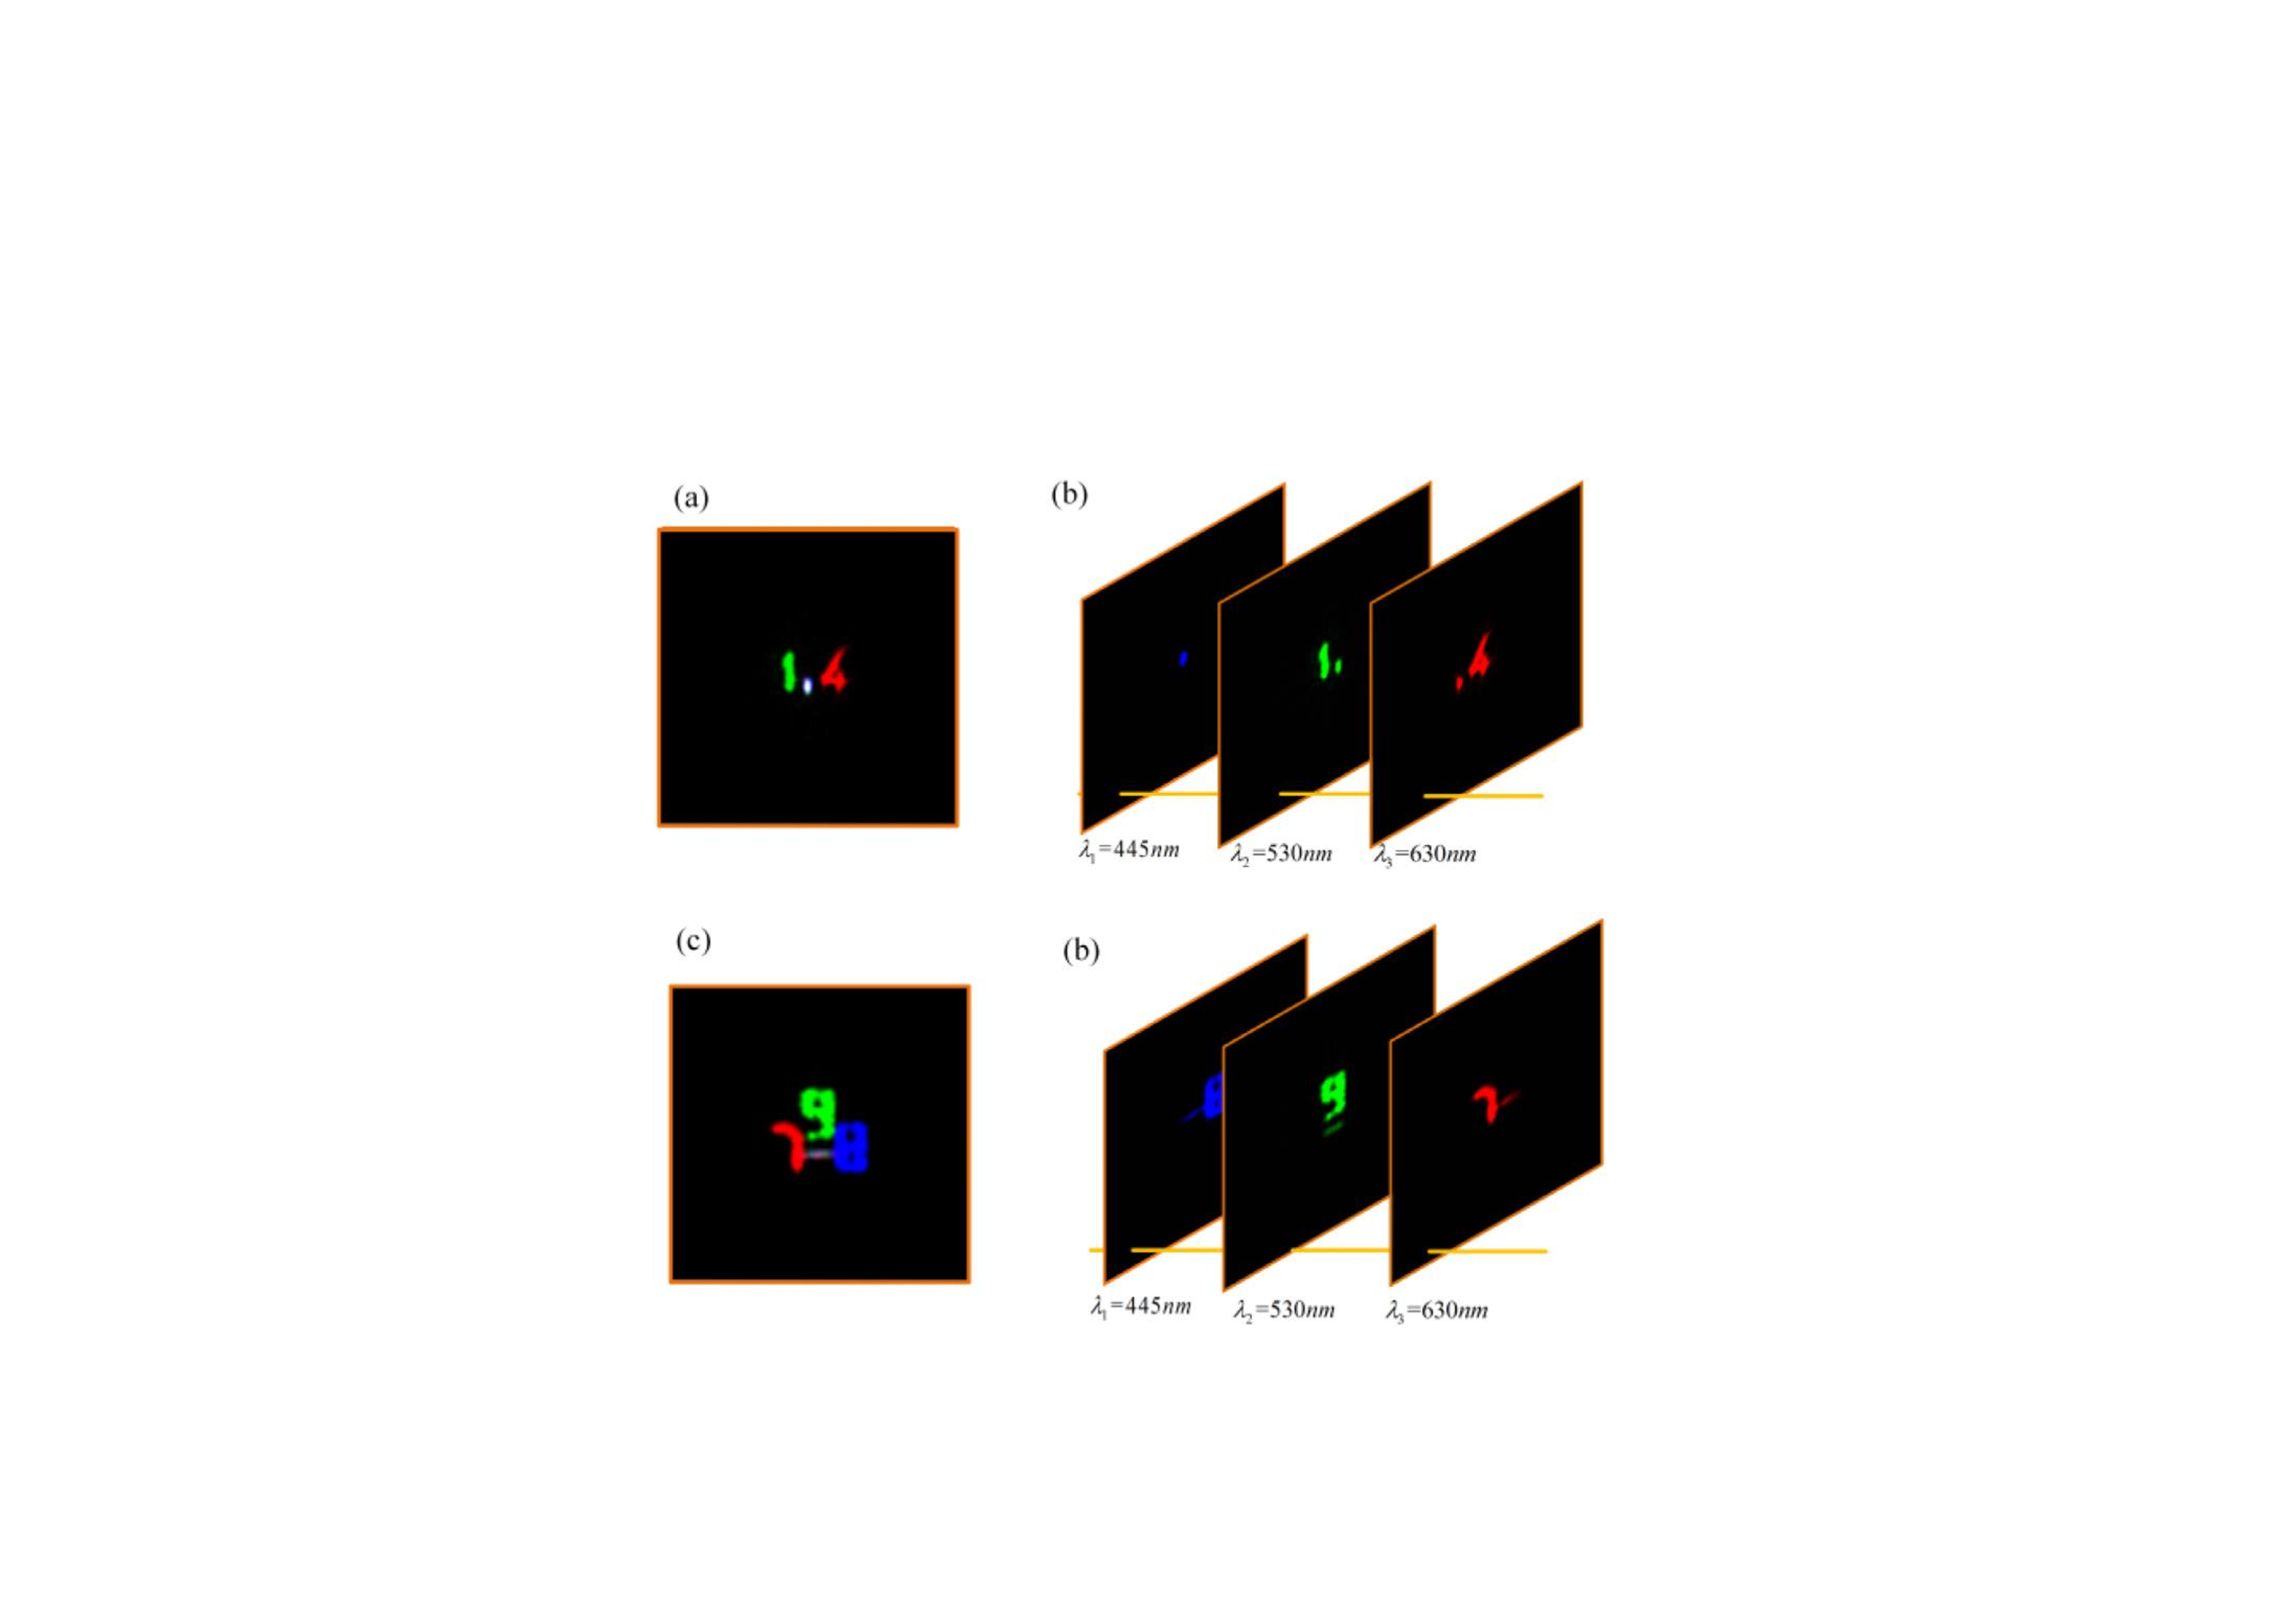
\includegraphics[scale=0.50]{C4.fig11}
	\caption{光谱成像实验结果}
	\label{fig:4.11}
\end{figure}

\subsection{成像分析}

在基于三阶相关的相位恢复算法中,我们需要将子散斑进行Radon变换,即将二维信号投影为$0\sim \pi$等分布的一维信号,然后进行三阶相位恢复。Radon变换时,所选取角度数量的多少会对最终的成像结果有所影响。在实验中,我们通常所采用的投影角度数量为18。为了更加直观的进行展示不同投影数所造成的最终影响,我们进行了相应的仿真,结果如图\ref{fig:4.12}所示。从图\ref{fig:4.12}(a-d)可以看出,随着投影数量的增加,成像质量也随之变高。当投影数量较少时,丢失了较多的傅里叶相位信息,导致不能较好的恢复图像。

\begin{figure}[htp]
	\centering
	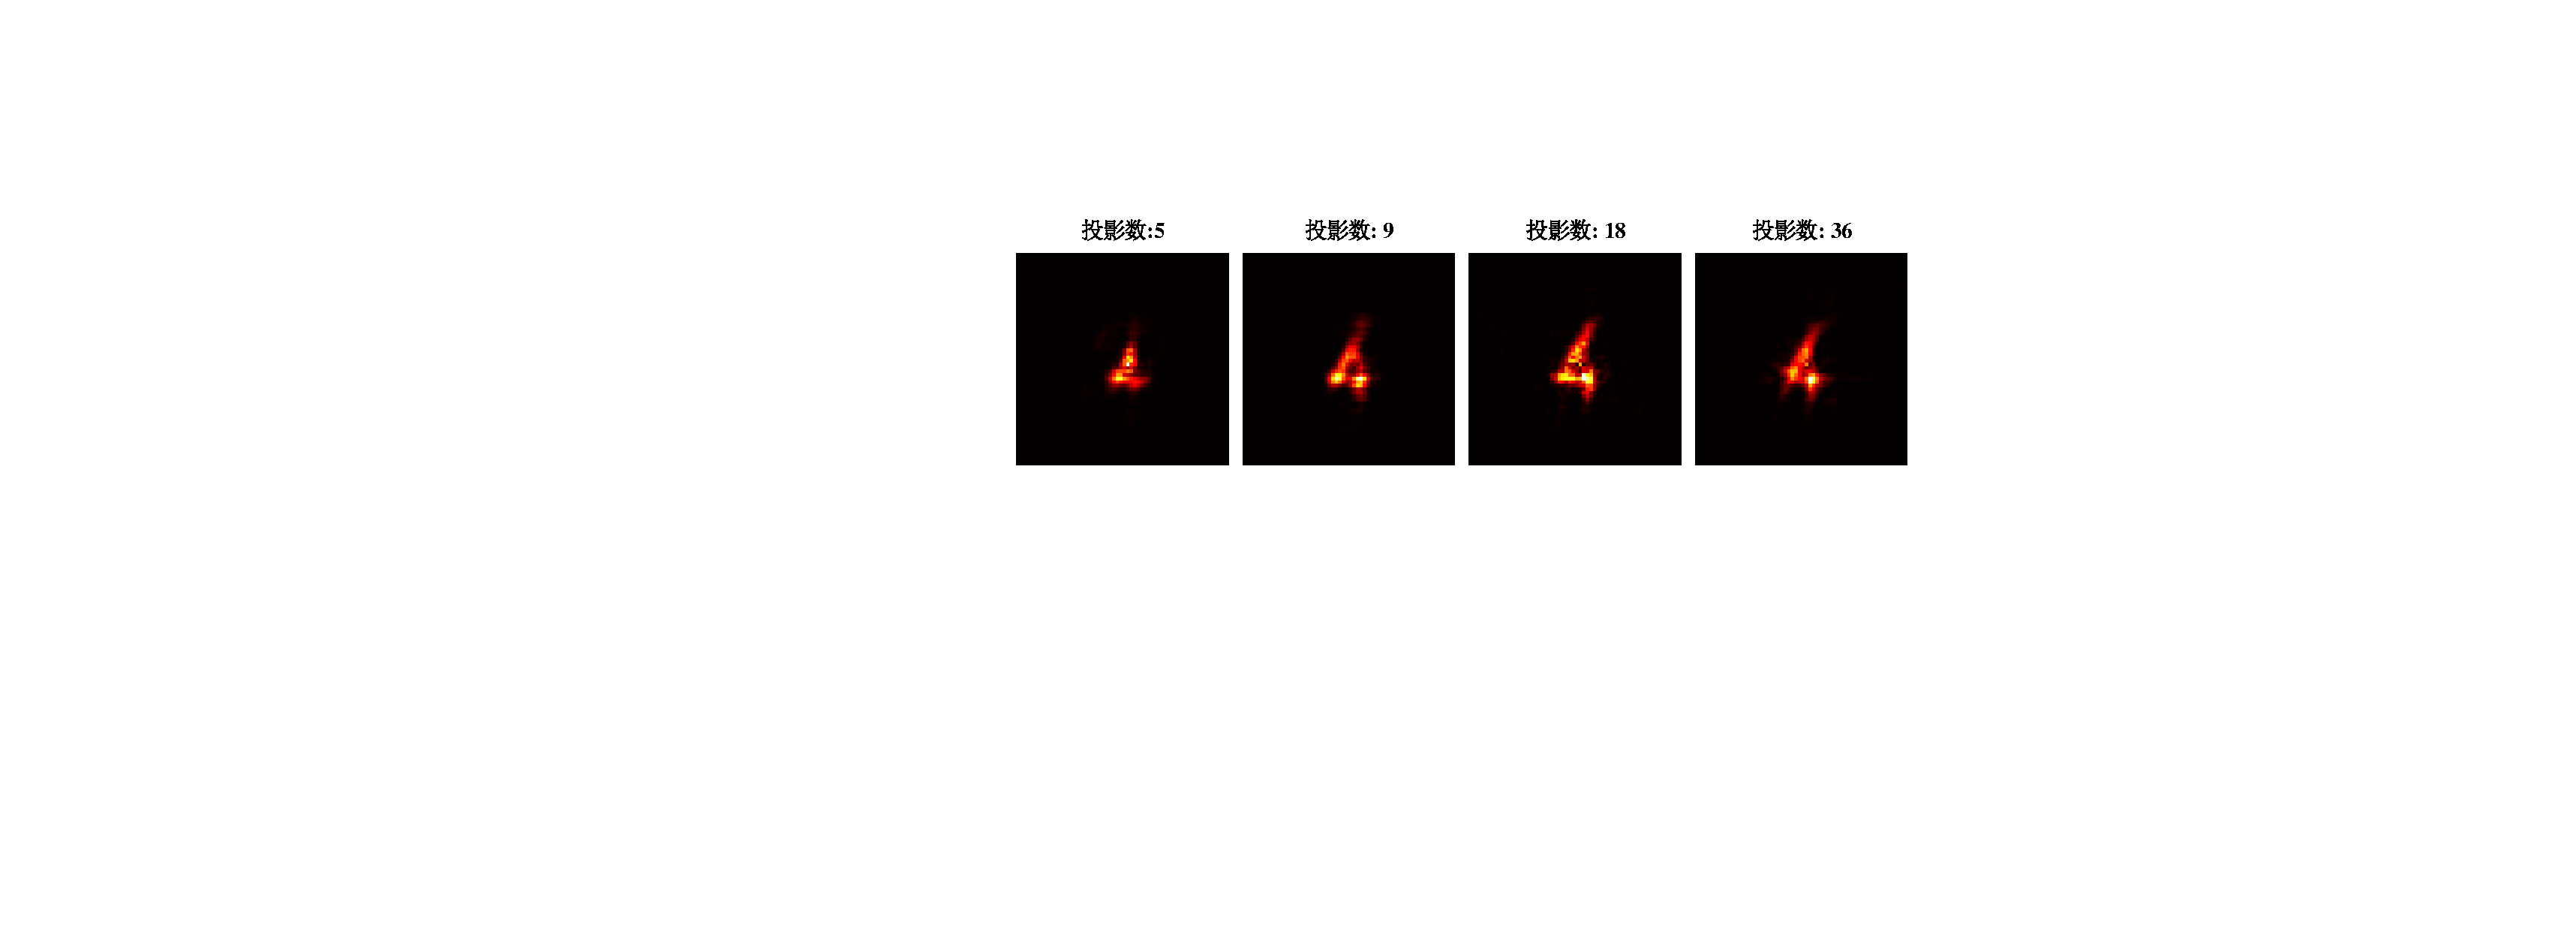
\includegraphics[scale=0.65]{C4.fig12}
	\caption{不同投影数的对比结果}
	\label{fig:4.12}
\end{figure}

与传统的散斑相关成像方法相比,基于三阶相关相位恢复算法所获取的相位信息与振幅信息获取步骤独立,不受到散斑自相关方法的振幅信息获取影响。传统的相位恢复算法所恢复的相位信息取决于已知的傅里叶振幅信息,当所获得傅里叶振幅信息不准确时,所恢复的傅里叶相位信息也将变得不准确。但是三阶相关相位恢复算法的相位恢复步骤与傅里叶振信息相互独立,在最终图像恢复方面具有更强的抗噪性能。我们进行了相关分抗噪性能分析,其实验结果如图\ref{fig:4.13}所示。具体实验步骤如下:首先,选取实验所获取的散斑;其次,加载不同级别功率的高斯白噪声至散斑图案(通过Matlab自带的awgn函数实现);其次,利用散斑图像重建算法实现图像重建。从图\ref{fig:4.13}可以看出,当信噪比大于10dB时,HIO和三阶相关相位恢复算法均能有效的重建目标;当信噪比小于10dB时,HIO不能恢复目标,三阶相关相位恢复算法仍能有效的重建目标。甚至,当信噪比为1dB时,三阶相关相位恢复算法仍能有效的重建目标。从实验结果可知,我们所使用的三阶相关相位恢复算法在透过散射介质成像方面有着较好的抗噪性能。

\begin{figure}[htp]
	\centering
	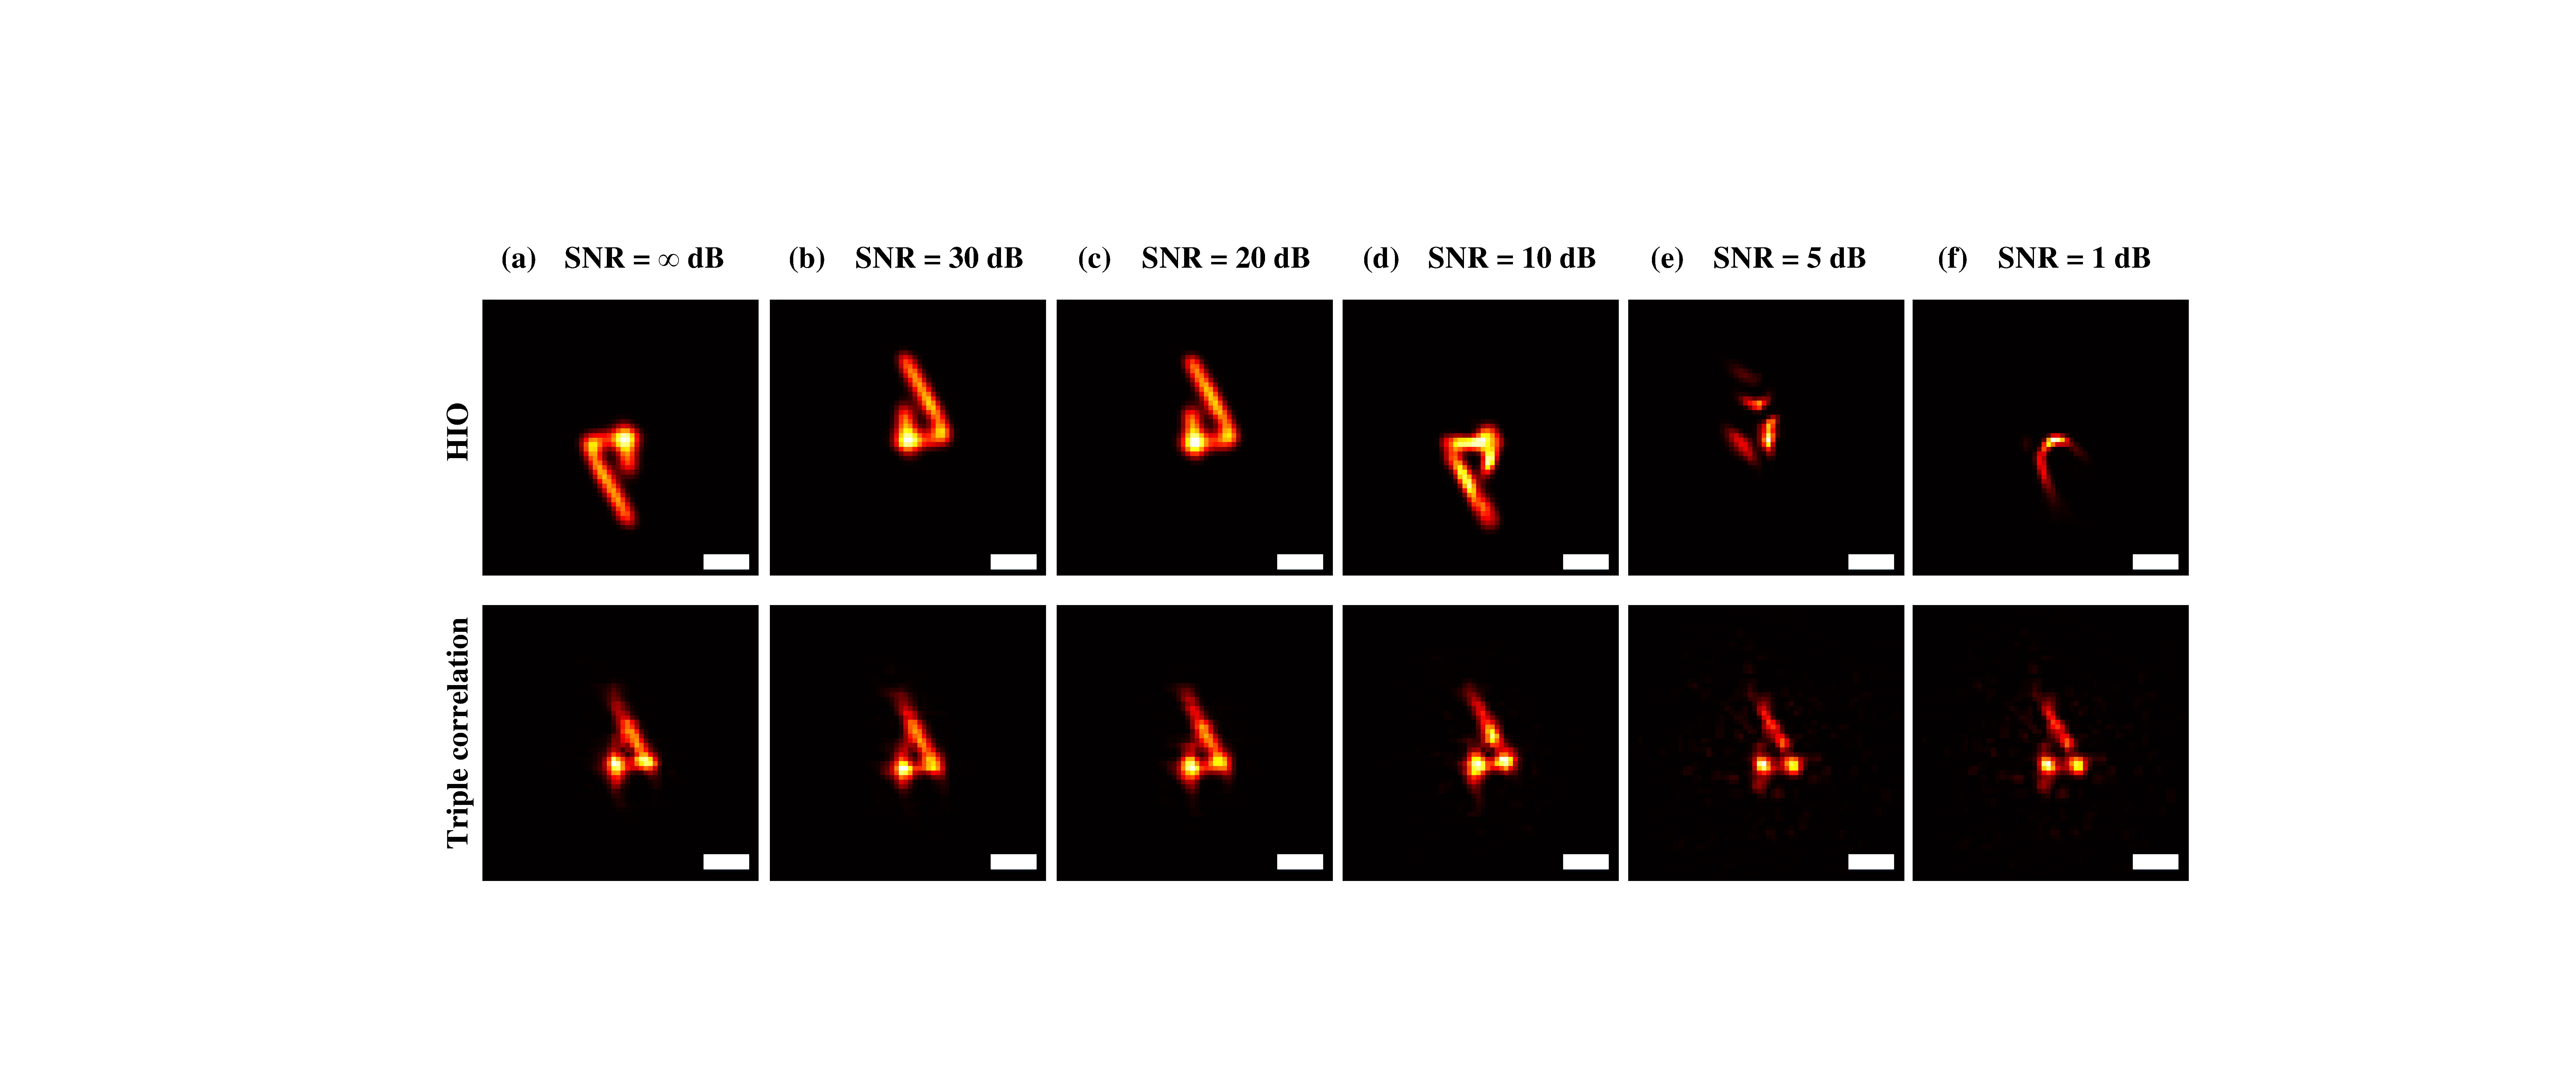
\includegraphics[scale=0.15]{C4.fig13}
	\caption{抗噪性能分析对比结果}
	\label{fig:4.13}
\end{figure}

在进行子散斑分割时,子散斑的尺寸应该接近于目标尺寸地2倍左右(单一轴),通常我们可以通过散斑地自相关来估计目标尺寸的大小。为了研究各个子散斑之间的重叠率对于最终重建的影响,我们尝试了子散斑重叠率分别为:$20\%$,$40\%$,$60\%$和$80\%$时所对应的重建结果,重建结果如图\ref{fig:4.14}所示。从图中可以看出,当重叠率为$80\%$时,隐藏目标可以被成功重建;当重叠率为$60\%$时,重建效果变差,但仍可以较完整的重建目标;当重叠率为$40\%$时,重建结果已经难以辨认;当重叠率减少至$20\%$时,重建目标为变得更为模糊。根据三阶相关相位恢复的理论可知,最终所恢复的相位需要通过对多帧子散斑的相位进行平均计算。该平均过程能够有效地抑制噪声,当子散斑重叠率变小时,对于噪声的抑制效果变差,导致最终重建结果变差,如图\ref{fig:4.14}(d3)所示;当子散斑之间的重叠率较高时,能够有效地对噪声进行抑制,获得更好地重建地结果,如图\ref{fig:4.14}(a3)所示。虽然随着重叠率减小,最终地成像质量变差。但是值得注意的是,虽然重叠率很低,但是重建结果仍然保持了隐藏目标地方向信息,如图\ref{fig:4.14}(d3)绿色轮廓所示。
从公式\ref{eq:4.16}可知,需要通过诸多子散斑之间的平均过程,消除不同子散斑所对应子孔径内所引入的散射效应。
同时从图\ref{fig:4.14}(a2)-(d2)可以看出,当子散斑之间重叠率较高时,我们能够获取较准确的傅里叶相位信息,极大的抑制噪声所;当子散斑之间的重叠率较低时,不够能较好的抑制噪声,相对获取误差较大的傅里叶相位信息,此处的实验结果也是对此理论的证明。

\begin{figure}[htp]
	\centering
	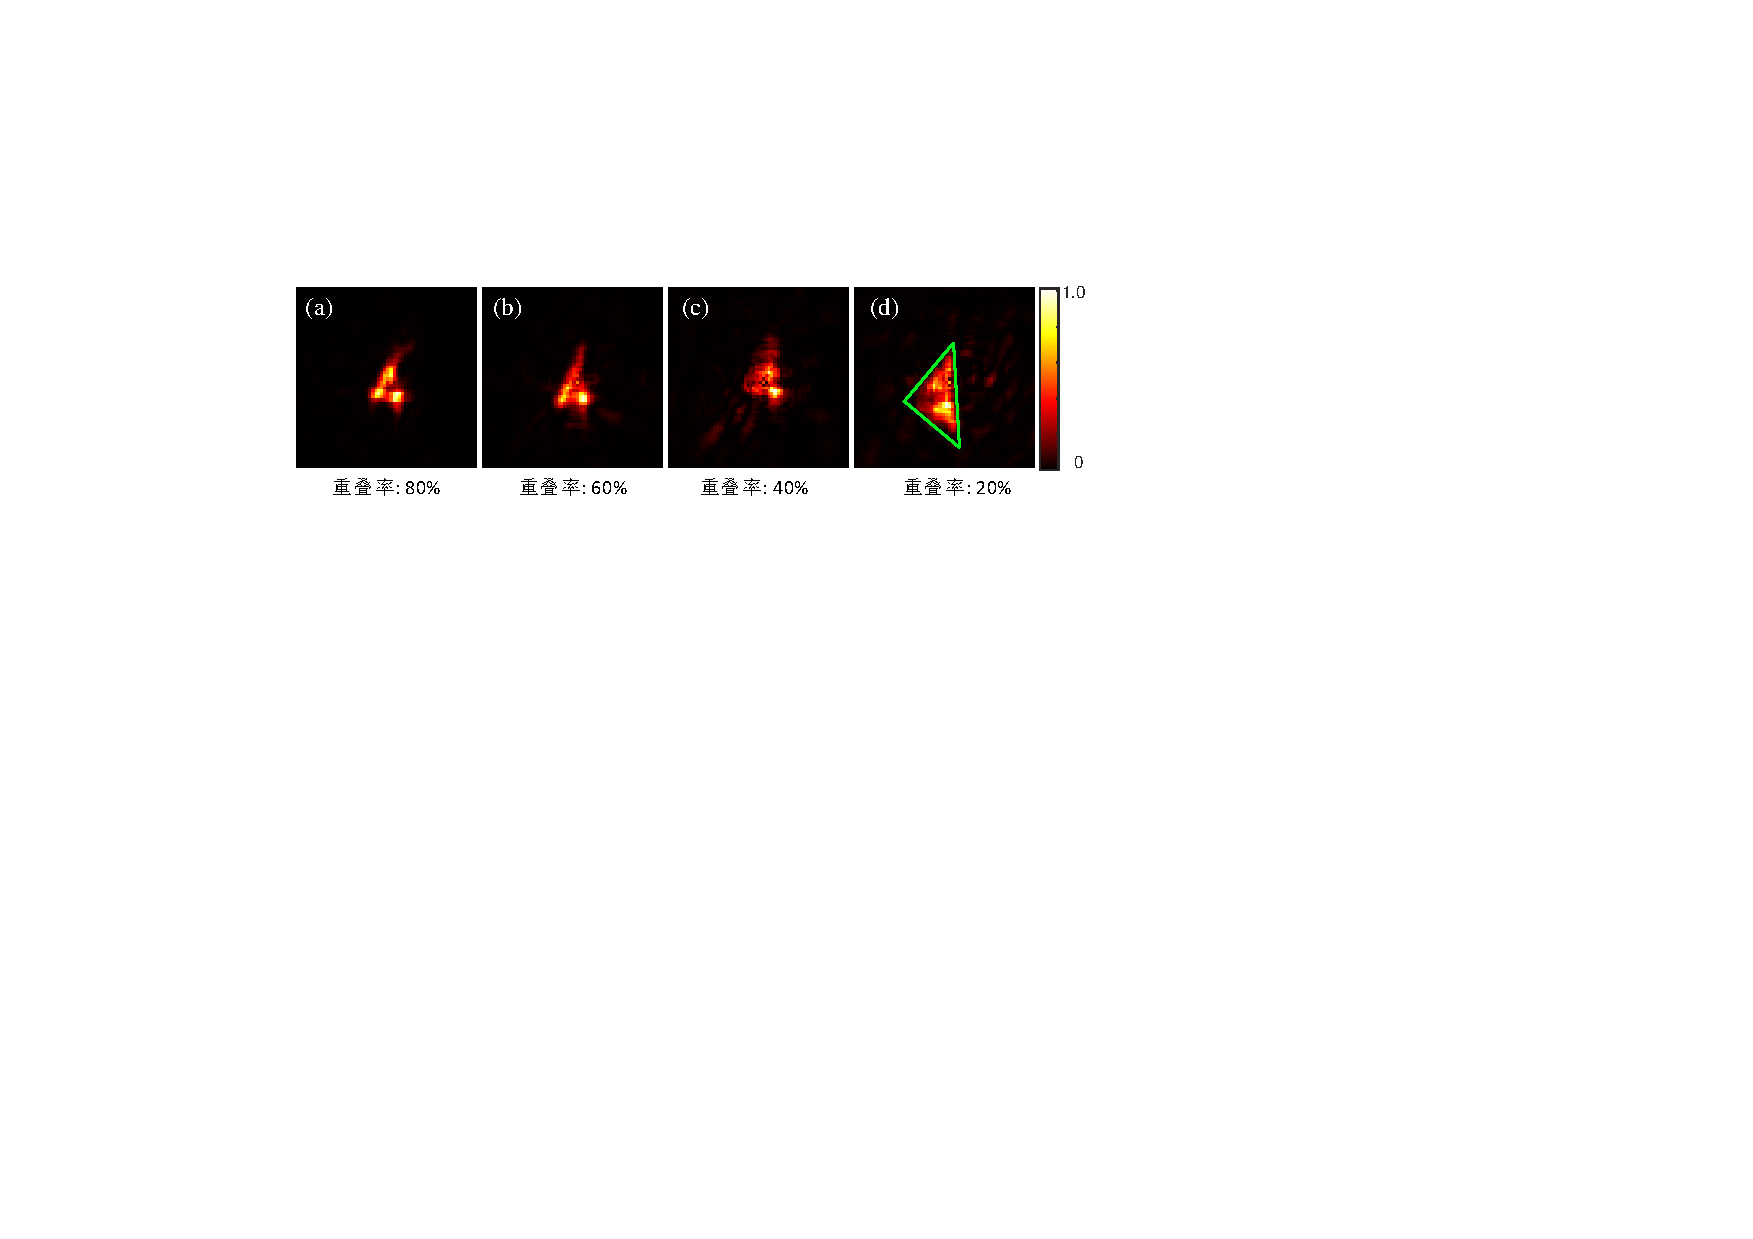
\includegraphics[scale=0.90]{C4.fig14}
	\caption{不同子散斑重叠率的重建结果}
	\label{fig:4.14}
\end{figure}

\section{基于三阶相关相位恢复方法扩展及讨论}

以上部分我们对于三阶相关相位恢复算法进行了介绍,并进行了相关实验,同时也实现了透过散射介质彩色成像的应用。但是仍有问题值得思考并讨论。

\subsection{不同相位恢复算法之间的混合}

在第三章节中,我们介绍了HIO和ER相位恢复算法,它们将傅里叶振幅作为输入信号,通过空域和频域的不同约束条件,进行迭代,实现最终的图像重建。它们的缺点在于无法保证有效地恢复目标,往往需要通过多次随机初始值尝试,最终选取满意地结果。同时,受到相位恢复原理的限制,不能够确定隐藏目标地方向信息。三阶相关相位恢复能够有效的有效地恢复目标的方向信息,但是为了获得较高的成像质量往往需要巨大的计算工作。我们尝试将三阶相关的相位恢复结果作为迭代型相位恢复算法的初始猜测,从而保证在确保有效恢复目标方向信息的同时,获得较高质量的重建图像。在此进行尝试之前,同样的我们需要解决另外一个问题:如何有效的结合HIO和ER相位恢复算法。在参考文献\cite*{bertolotti_non-invasive_2012,katz_non-invasive_2014}中,将HIO算法的迭代优化结果作为ER相位恢复的初始值,然后进行迭代优化以获得最终结果。我们是否可以将HIO算法和ER算法进行有机的结合,在单次的迭代中同时使用HIO和ER算法?我们将在下面部分分别进行尝试。方法一:将基于三阶相关的相位恢复算法的恢复结果作为HIO算法的初始猜测进行迭代,当HIO获取最终结果后,将其结果作为ER算的的初始值进行迭代优化获得最终结果,其原理如图\ref{fig:4.15}所示。利用次混合相位恢复算法,进行相应的图像重建。方法二:将基于三阶相关的相位恢复算法的恢复结果作为HIO算法的初始猜测进行迭代,在单次迭代中将HIO的输出作为ER的输入进行优化,并将ER的输出再次传递给HIO进行下一次迭代优化,直至获得最终结果,其原理如图\ref{fig:4.16}所示。
混合型算法\Romannum{1}和\Romannum{2}所对应的实验结果如图\ref{fig:4.17}所示,所有的恢复结果均来同一散斑,图\ref{fig:4.17}(a)-(c)为混合型相位恢复算法\Romannum{1}的实验结果,图\ref{fig:4.17}(d)-(f)为混合型相位恢复算法\Romannum{2}的实验结果。从图\ref{fig:4.17}中可以看出,混合型相位恢复算法\Romannum{1}和\Romannum{2}所重建图像的质量较为接近,但是混合型相位恢复算法\Romannum{1}不能确保目标的方向信息,混合型相位恢复算法\Romannum{2}可以保证恢复目标的方向信息。
同时为了直观的对比不同算法之间图像重建的差异,图\ref{fig:4.17}(f)-(h)为基于三阶相关的相位恢复算法所重建的结果。可以看出,混合型算法的重建图像质量明显优于原始三阶相关的相位恢复算法所重建图像质量。基础的三阶相关的相位重建算法给混合型相位算法提供了较准确的初始相位猜测,HIO和ER算法能够有效地利用较准确的相位初始猜测恢复图像。但是值得注意的是,混合型算法\Romannum{1}不能确保恢复目标的方向信息,混合型算法\Romannum{2}可以恢复目标的方向信息。
\begin{figure}[htp]
	\centering
	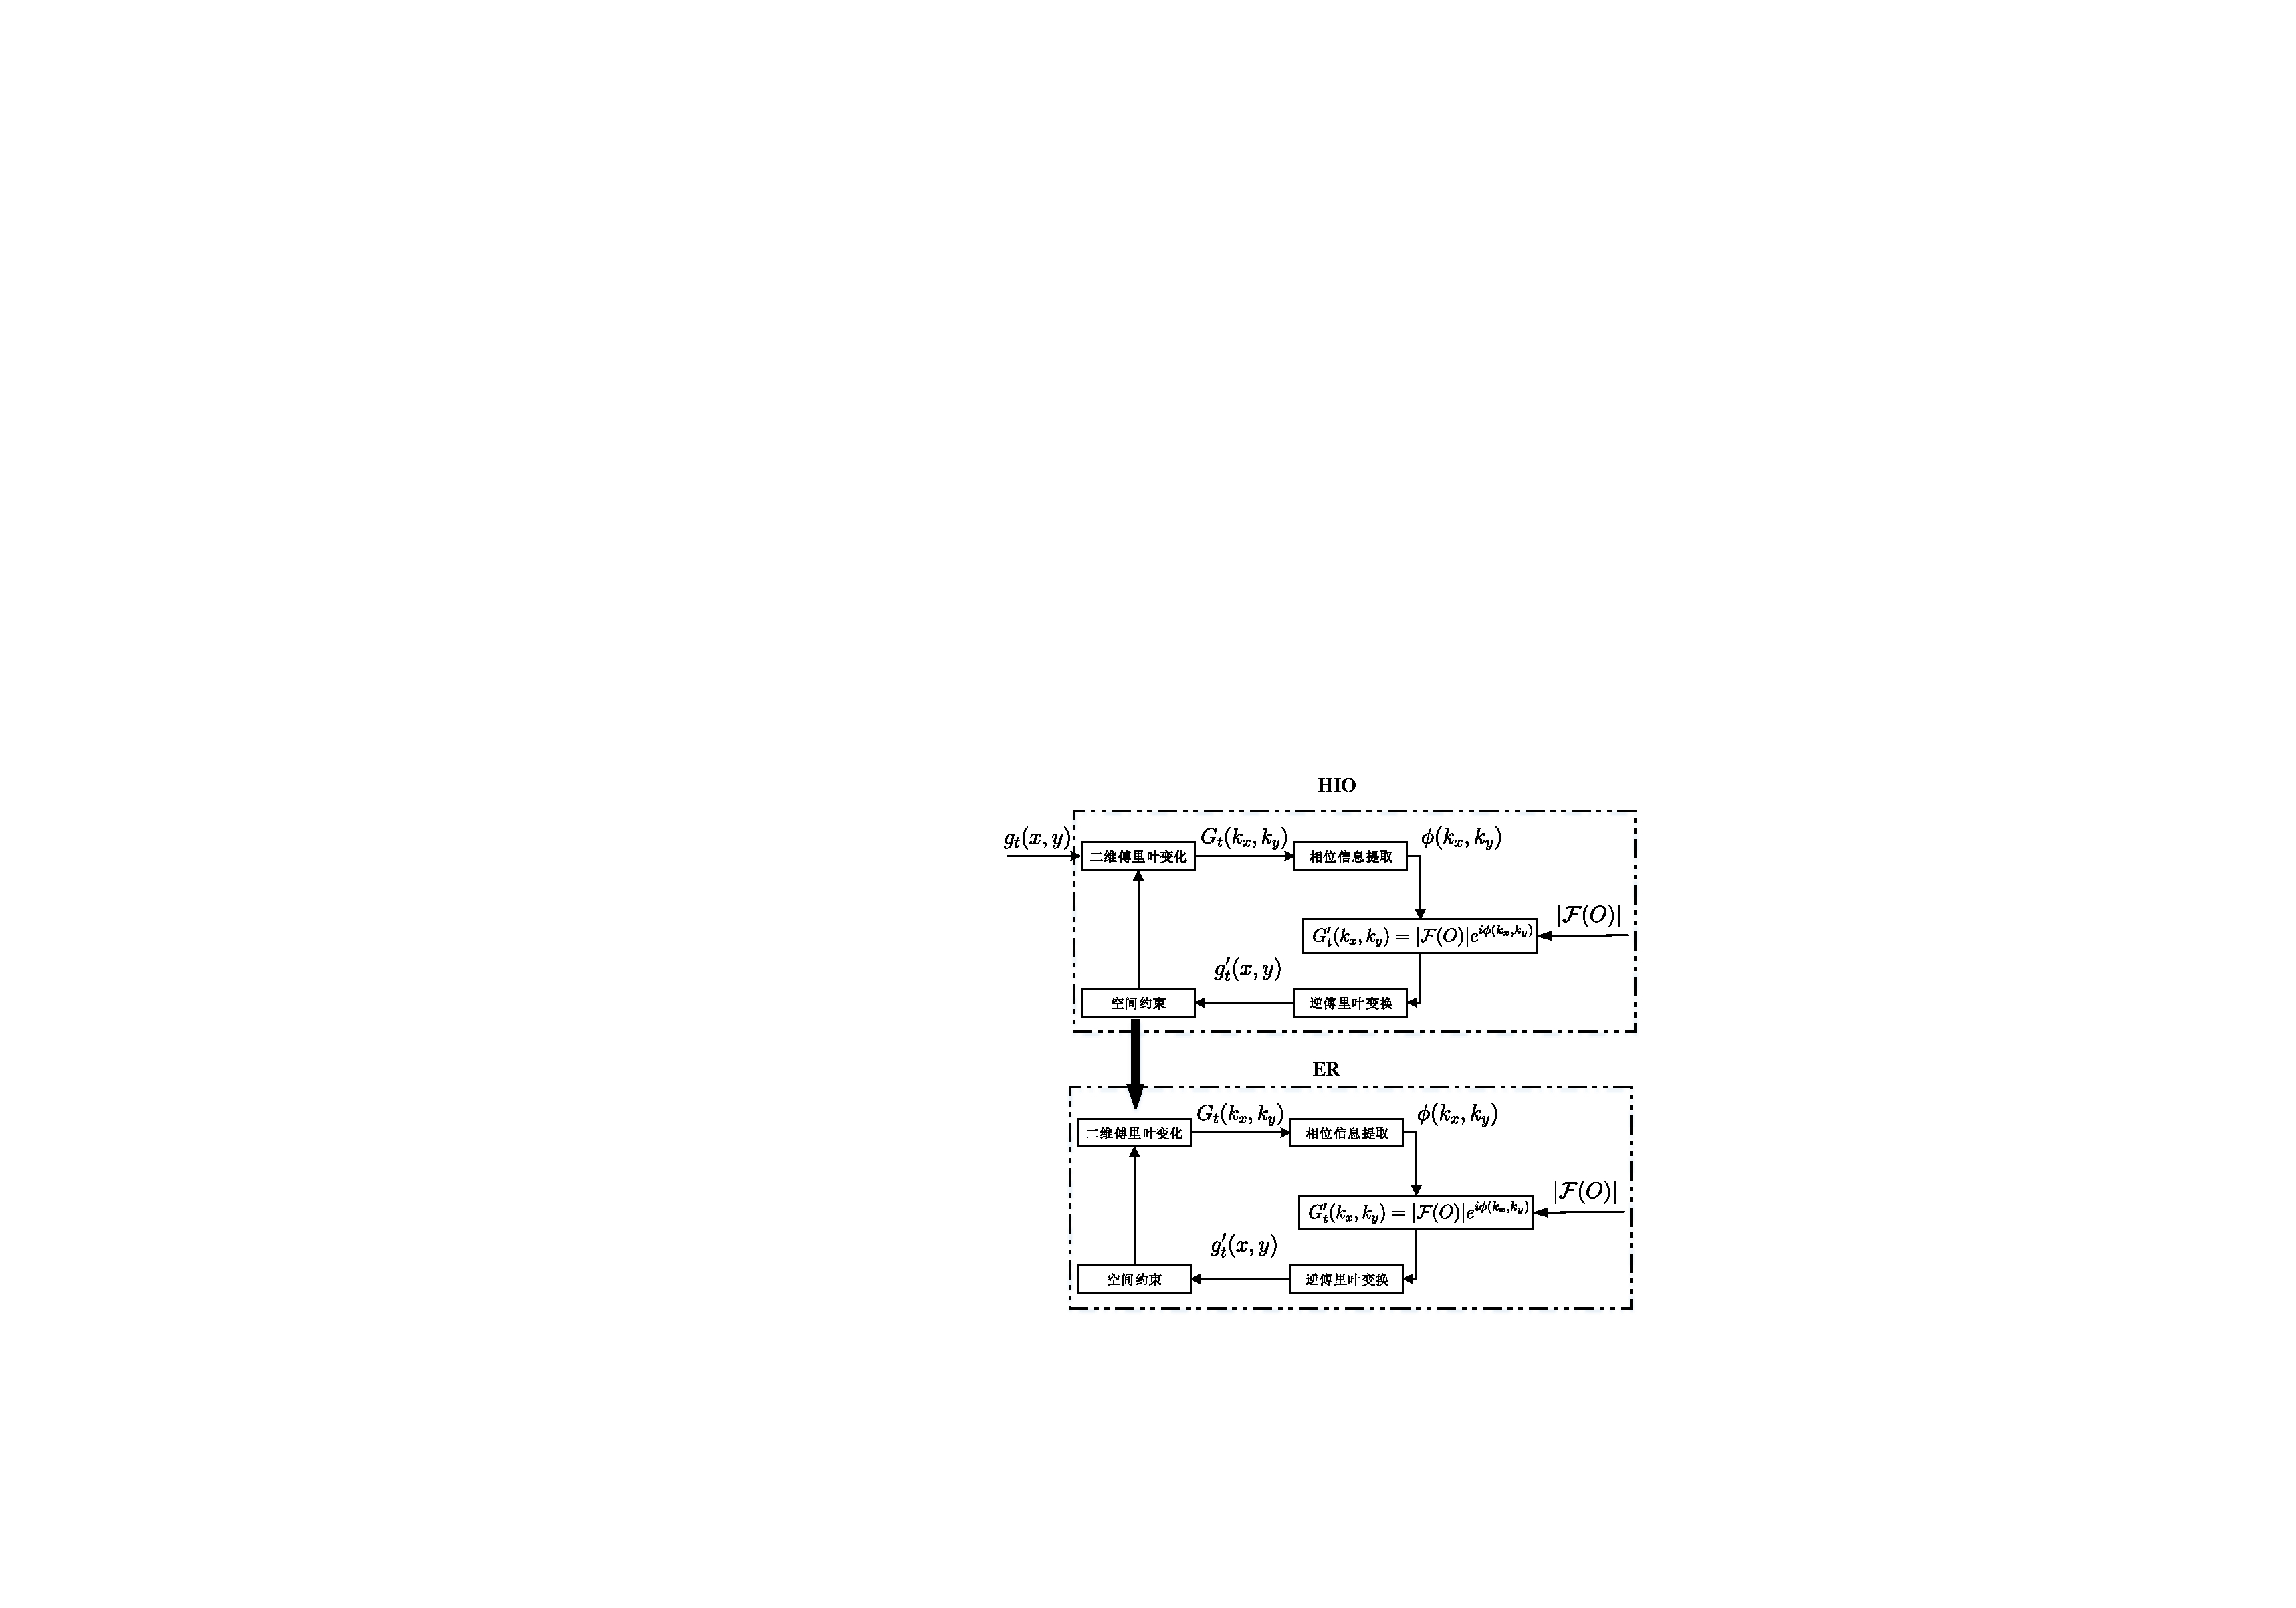
\includegraphics[scale=0.70]{C4.fig15}
	\caption{混合型相位恢复算法\Romannum{1}}
	\label{fig:4.15}
\end{figure}

\begin{figure}[htp]
	\centering
	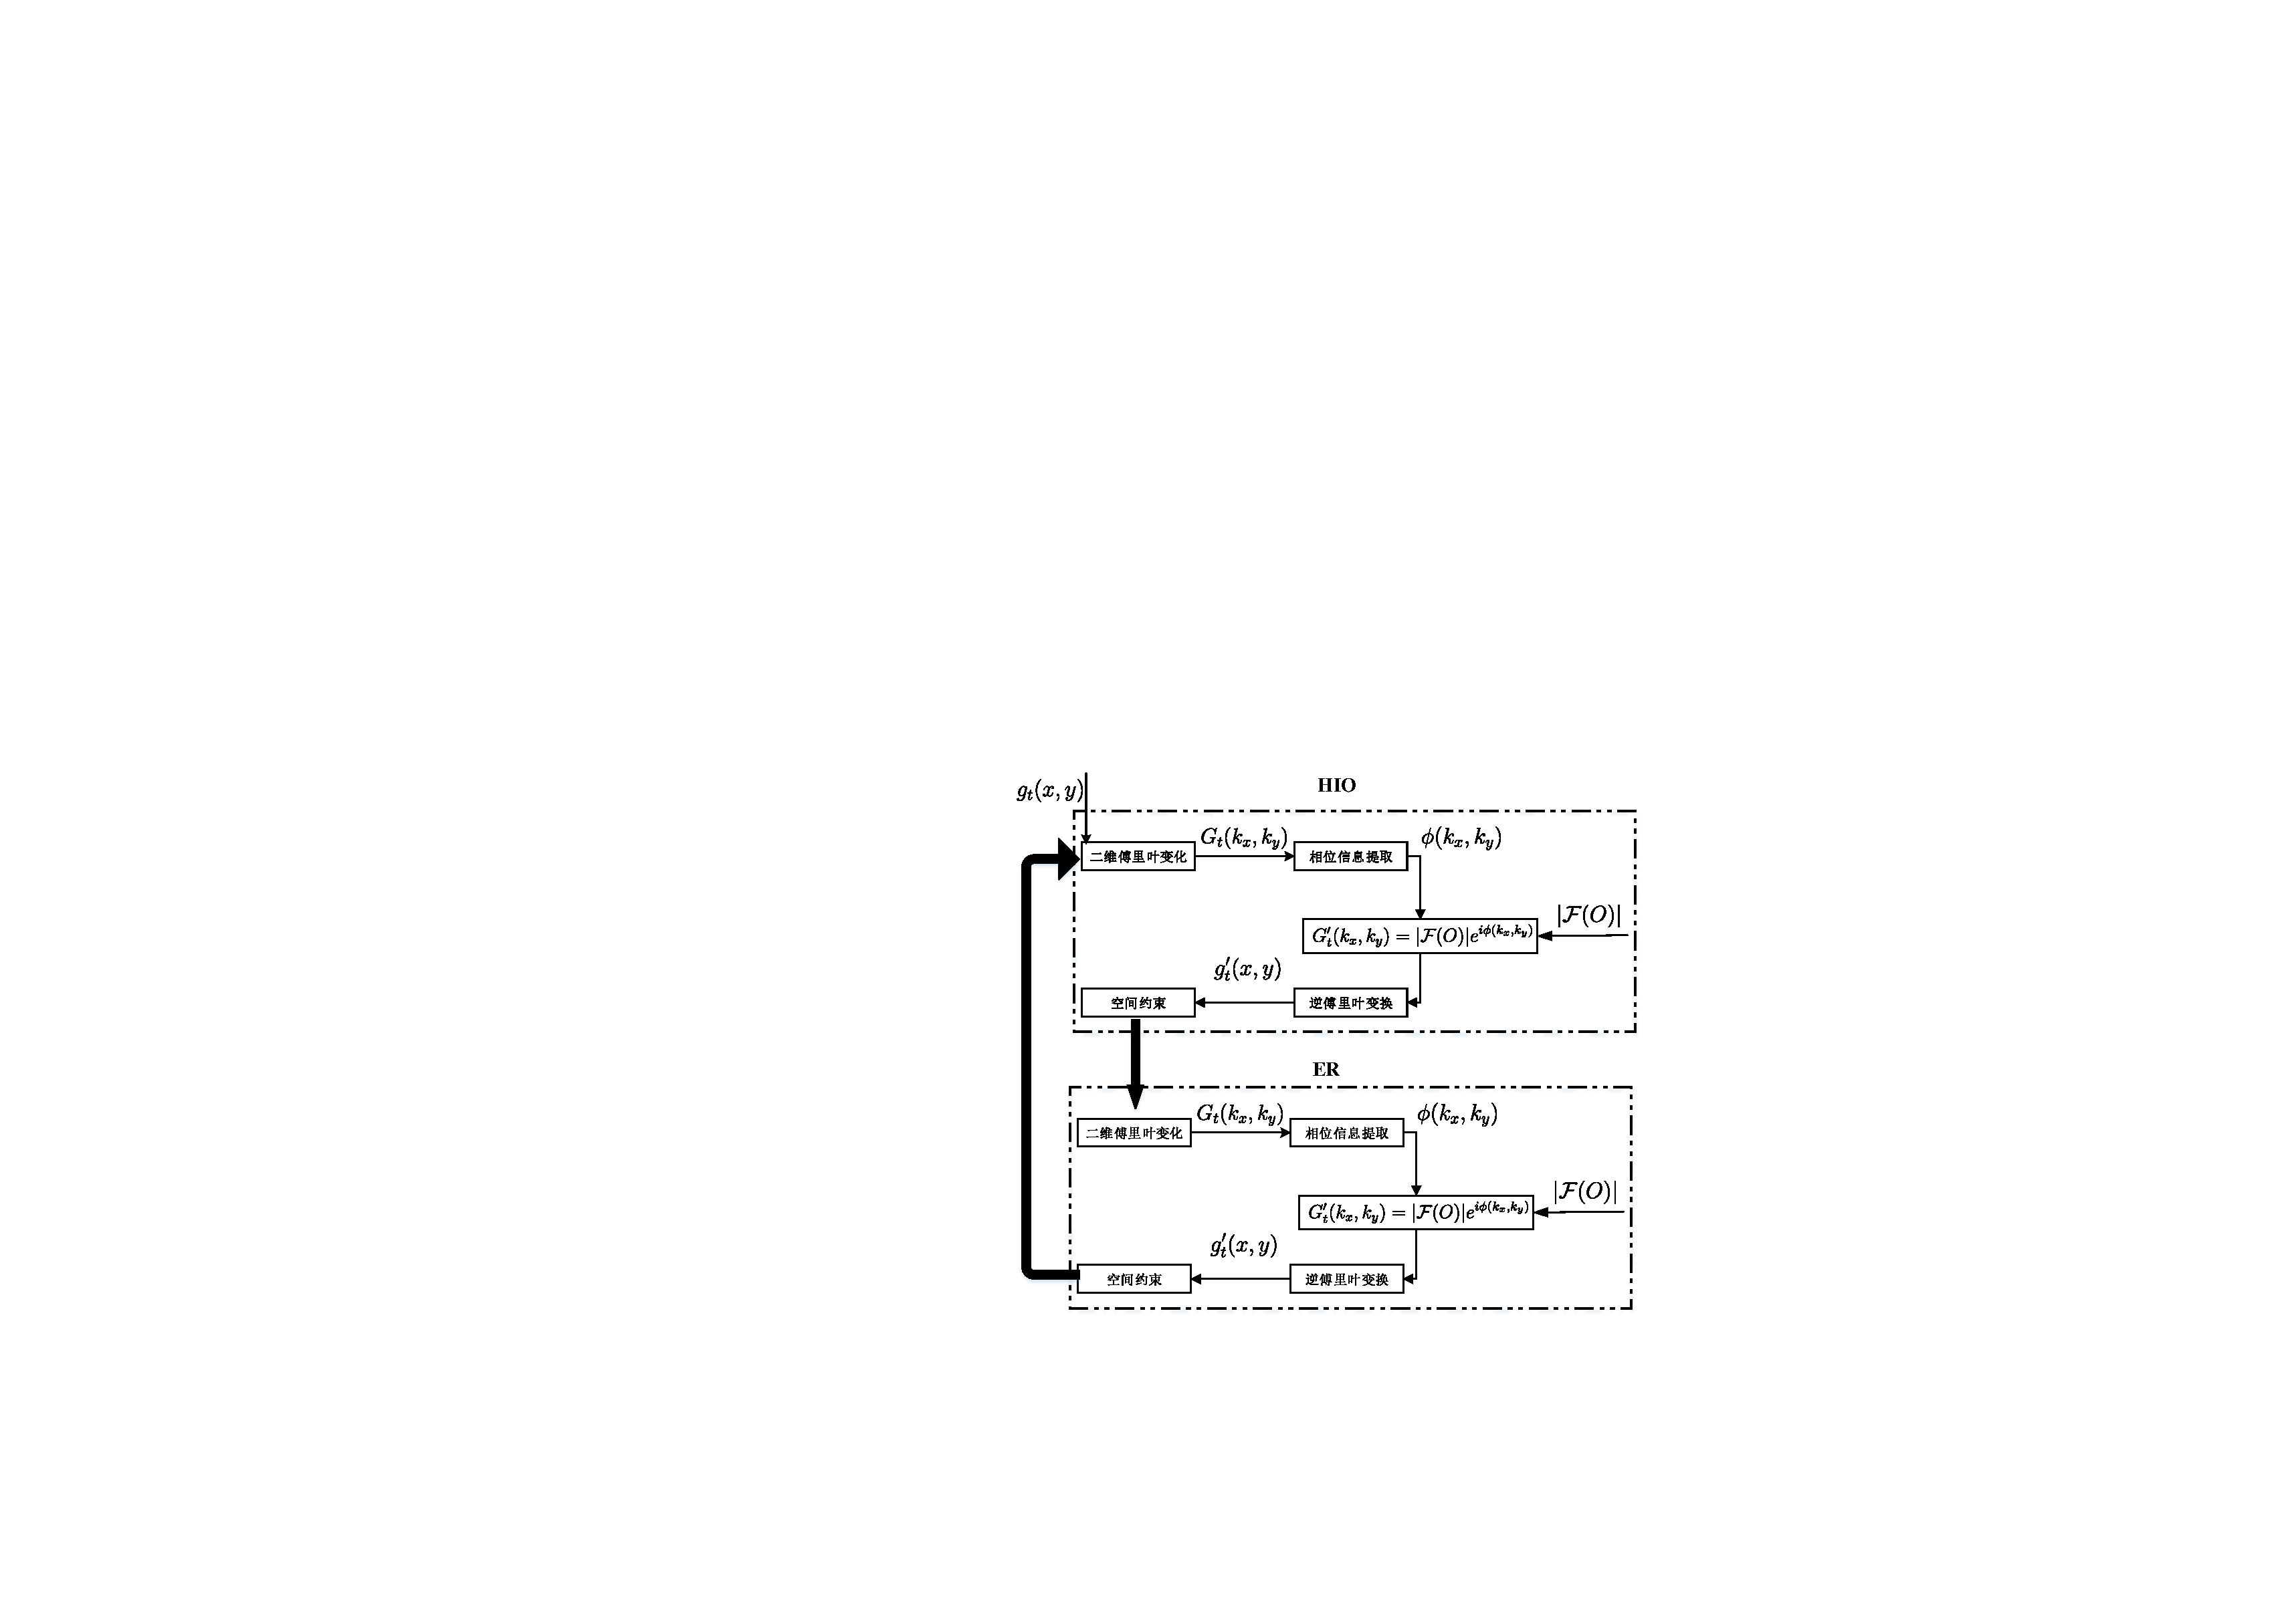
\includegraphics[scale=0.70]{C4.fig16}
	\caption{混合型相位恢复算法\Romannum{2}}
	\label{fig:4.16}
\end{figure}


\subsection{噪声分析}
为了分析噪声对于三阶相关相位恢复算法的影响,我们进行了以下简要分析。

情况\romannum{1}:三阶相关与加性噪声。
我们为了简化分析噪声对于三阶相关相位恢复的影响,假设信号$S(x)$由信号$I(x)$和独立的加性噪声$N(x)$构成,即
\begin{equation}
\begin{aligned}
S(x) = I(x)+N(x)
\end{aligned}
\label{eq:4.20}
\end{equation}其中,$\langle N(x) \rangle = \mbox{常数} $,$\langle N(x^{\prime})  N(x^{\prime} +x) \rangle = N^{(2)}(x) $
信号$S(x)$的平均相关为:
\begin{equation}
\begin{aligned}
\langle S^{(3)}(x) \rangle = & \underbrace{I^{(3)}(x)}_{\text{[0]}}+\\
& \underbrace{\langle N(x)\rangle \cdot \left[ I^{(2)}(x) +I^{(2)}(x^{\prime}) +I^{(2)}(x^{\prime}-x) \right] }_{\text{[1]}}+\\
& \underbrace{ \bar{I} \cdot \left[ N^{(2)}(x) +N^{(2)}(x^{\prime}) +N^{(2)}(x^{\prime}-x) \right]}_{\text{[2]}}+\\
& \underbrace{\langle N^{(3)}(x)\rangle}_{\text{[3]}}
\end{aligned}
\label{eq:4.21}
\end{equation}其中,$N^{(2)}(x) = \int N(x_1) \cdot N(x_1+x) \mathrm{d}{x_1}$,$\bar{I} = \int I(x)\mathrm{d}{x}$。

当信号为加性噪声时,平均后三阶相关的噪声包含三项:第一项为$S(x)$的自相关加和,第二项为$N(x)$的自相关加和,第三项为$\langle N^{(3)}(x)\rangle$,通常此项为零值。

\begin{figure}[htp]
	\centering
	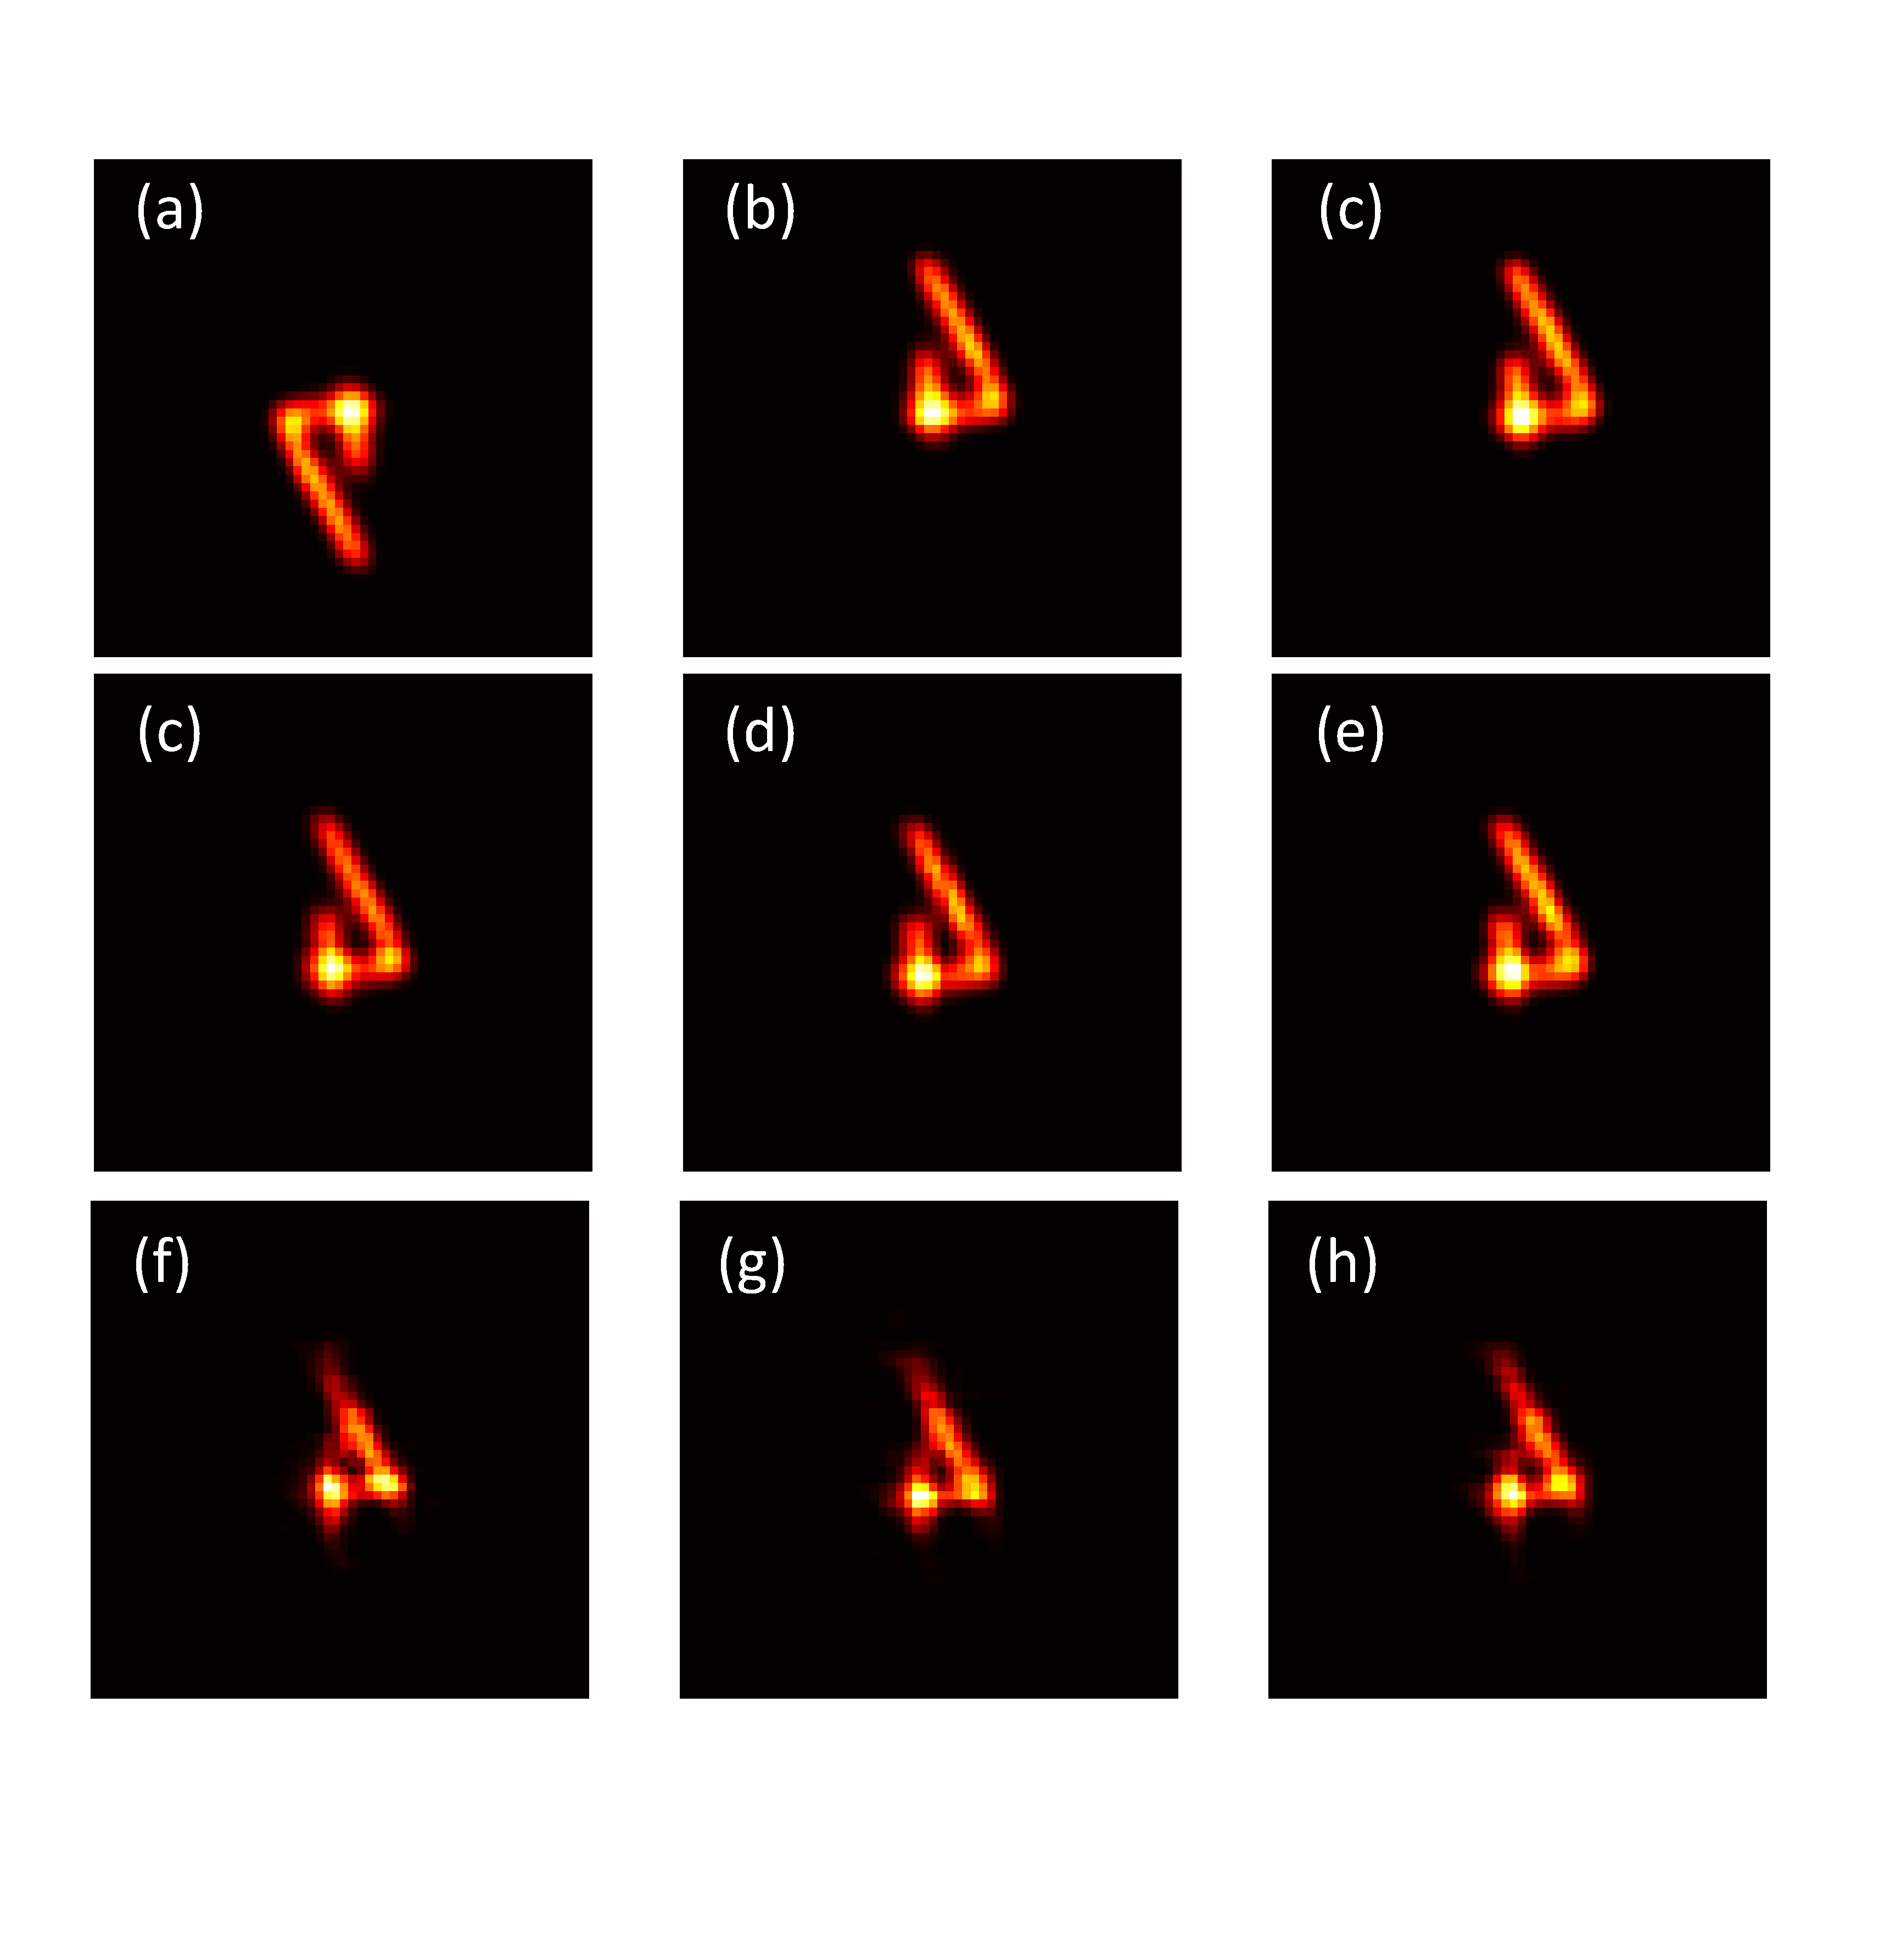
\includegraphics[scale=0.15]{C4.fig17}
	\caption{不同相位恢复算法的实验结果}
	\label{fig:4.17}
\end{figure}

情况\romannum{2}:如参考文献\cite{lohmann_speckle_1983,wu_single-shot_2016}所指出,计算三阶相关能够有效的抵消引因为大气湍流或者抖动引起的随机相位,对于整个孔径来说,仍存在许多不可分的子孔径。当在相关计算中,计算位于同一闭合相位中的频率时,能够有效的抵消随机相位,此时不会差生噪声。当相关的频率位于不同的闭合三角形中时,不能有效的抵消随机相位,同时会产生不同种类的噪声。

如我们所知,三阶相关相位恢复算法需要通过多帧子散斑平均地方式实现相位恢复,如图\ref{fig:4.14}所示,子散斑之间的不同重叠率将会影响最终的相位重建结果。直观来看,子散斑之间的不同重叠率直接影响子散斑的数量,子散斑的数量将会影响最终重建结果。同理,原始散斑的尺寸也会影响子散斑的数量,也会对最终的重建结果进行影响。我们从统一散斑中选取不尺寸的散斑作为原始散斑图案,并进行重建,结果如图\ref{fig:4.18}所示。从实验结果可以看出,当选择尺寸较大散斑时,三阶相关相位恢复算法能够更好的抑制噪声,获得更高质量的重建图像。

\begin{figure}[htp]
	\centering
	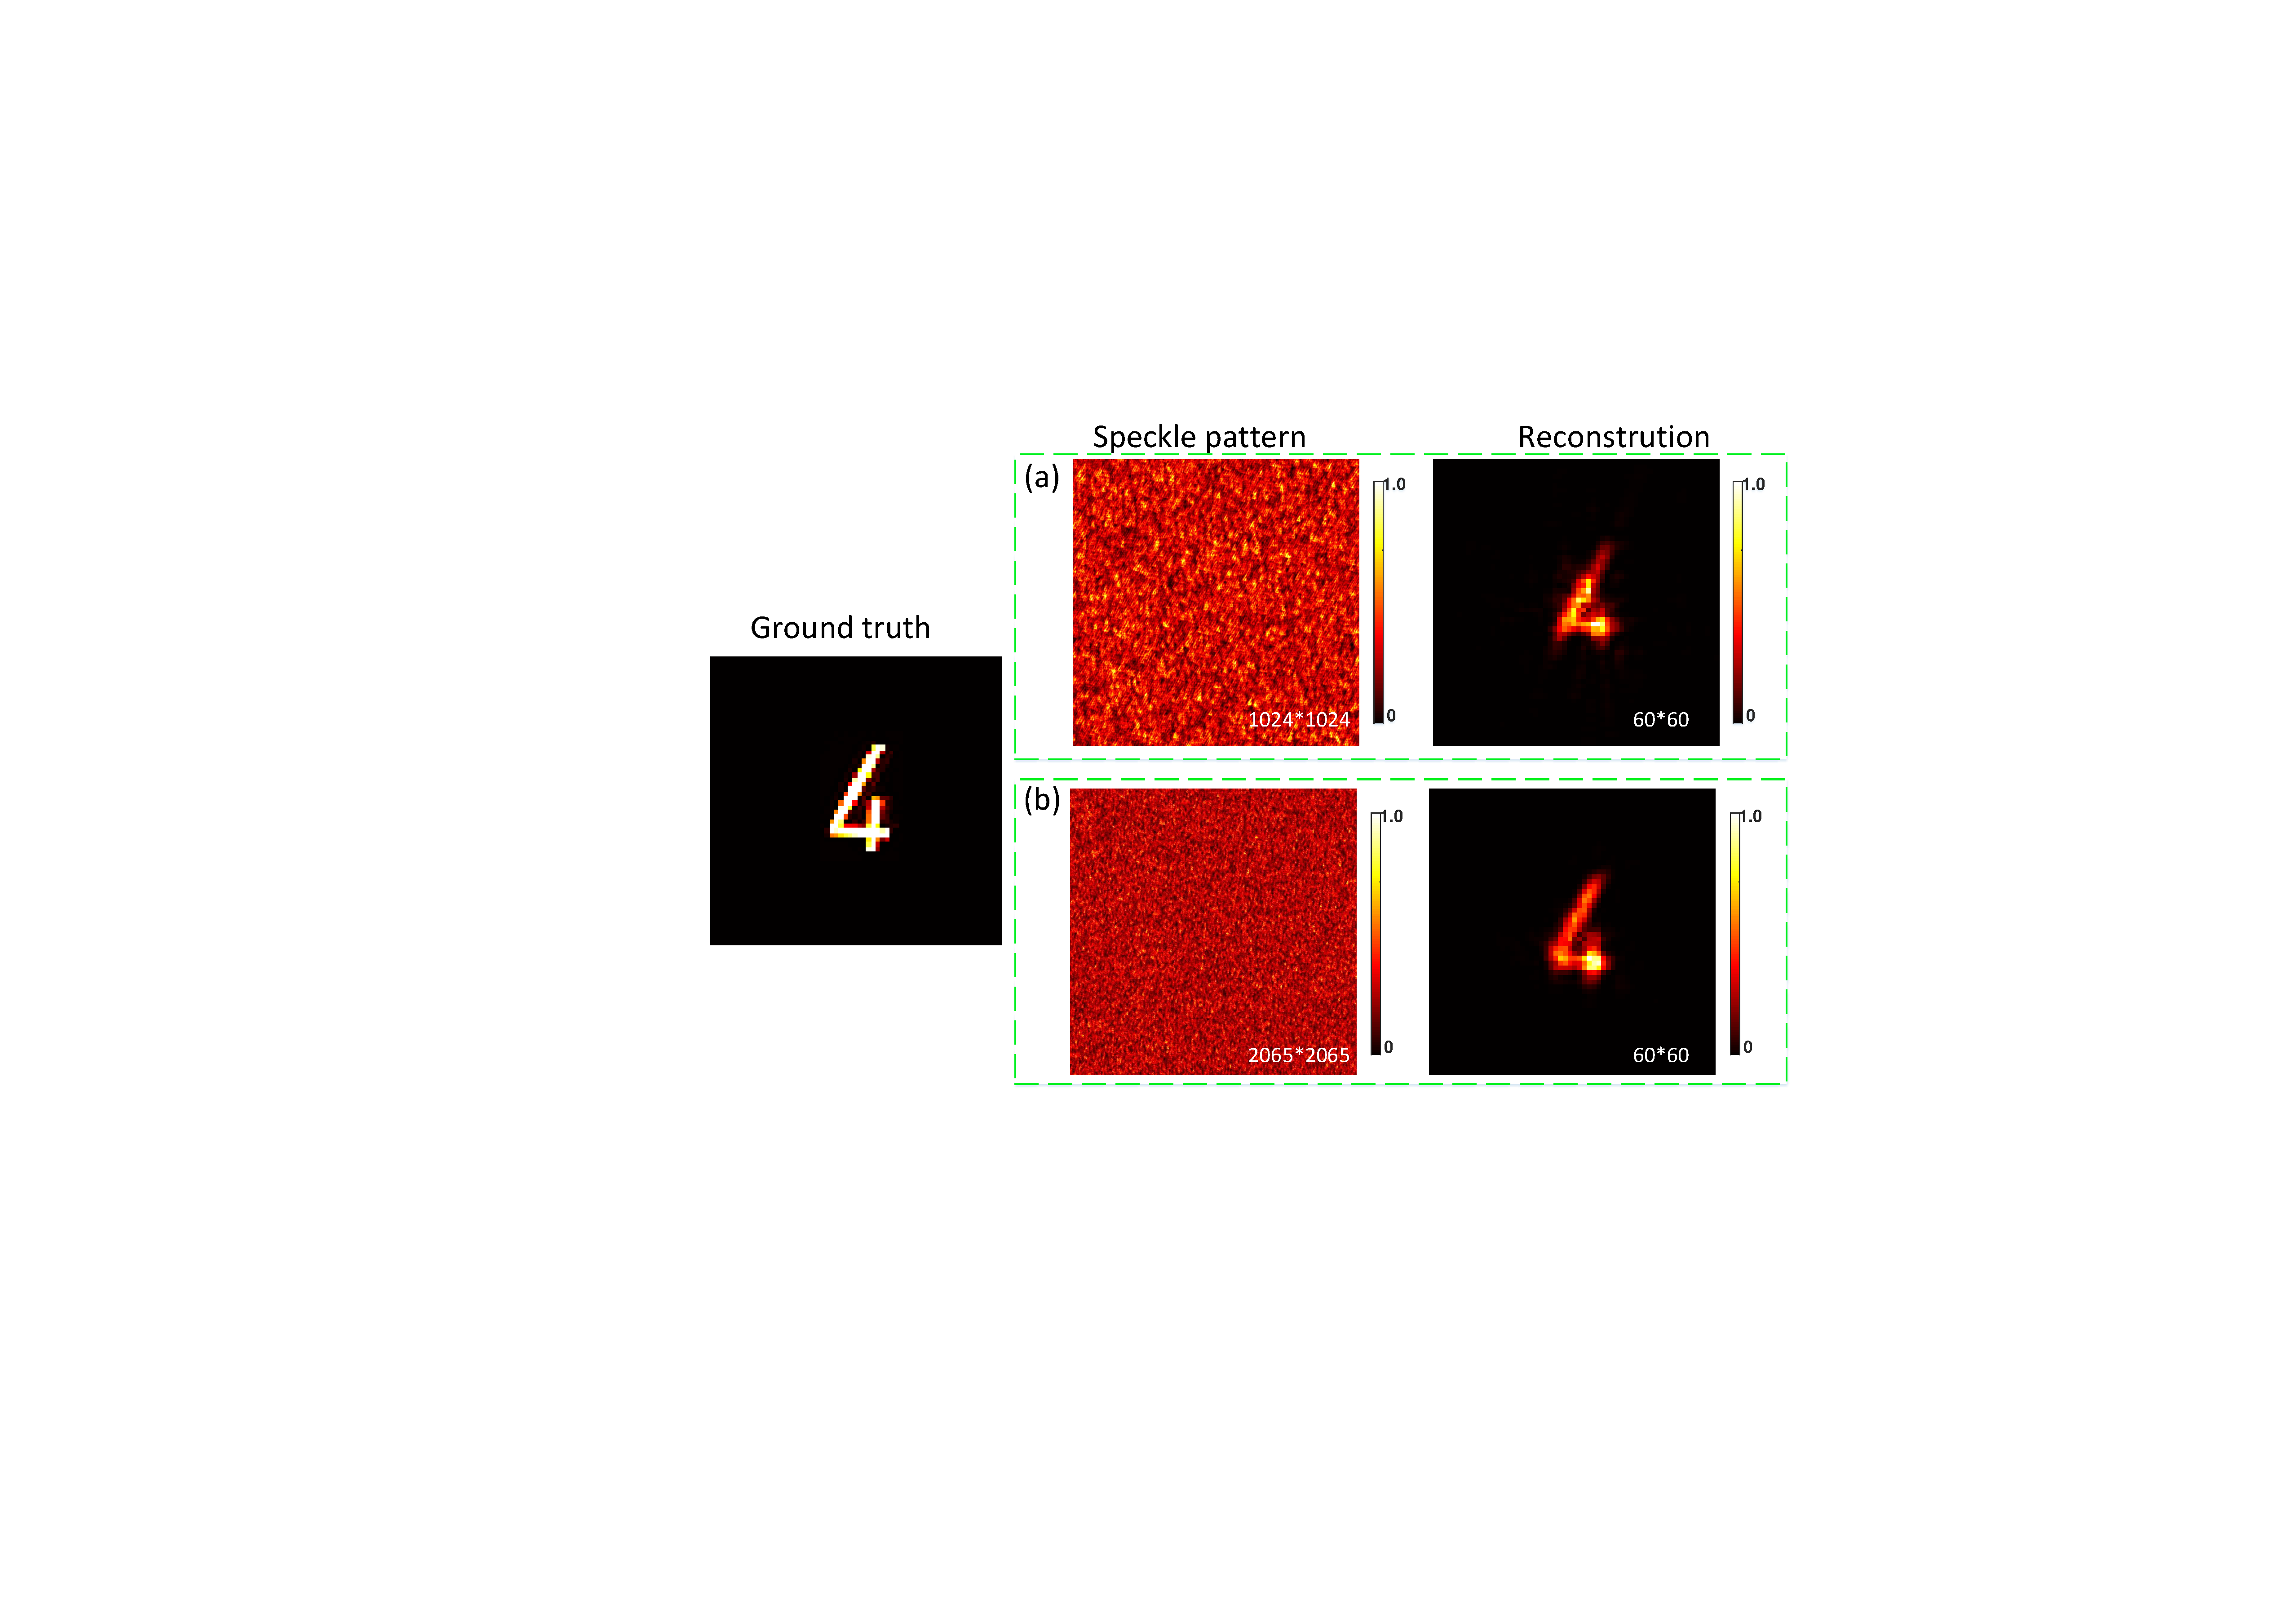
\includegraphics[scale=0.25]{C4.fig18}
	\caption{不同尺寸散斑的重建结果}
	\label{fig:4.18}
\end{figure}
\section{本章小结}

本章中,我们提出了基于三阶相关相位恢复算法的透过散射介质彩色成像方法,利用三阶相关的相位恢复算法的特性,实现了透过散射介质彩色成像。相较于传统的透过散射介质成像方法,该方法能够有效的确保恢复目标的方向信息,并利用此特性进行彩色图像合成。基于三阶相关相位恢复算法,不需要迭代,能够确定性的恢复相位。同时,该方法的傅里叶相位恢复步骤与傅里叶振幅恢复步骤相会独立,相较于传统迭代型相位恢复算法具有较强的抗噪性能。我们也讨论了不同相位恢复算法之间的混合,通过实验证明了有效地进行混合能够确保混合型算法在确保恢复目标方向信息的同时提高图像的重建质量。我们所提出的彩色成像方法,能够与传统的光谱成像方法结合,通过添加参考目标的方式,有助于实现透过散射介质的光谱成像,该方面我们也通过实验的方式进行了简单证明。

本章所进行的工作基础,仍然利用基于OME。所以我们的成像范围仍然受到OME范围的限制,如何进行突破OME范围,实现超OME且完全非入侵成像仍是不可避免地问题。下一章我们将介绍如何实现非入侵透过散射介质成像,并且同时实现超OME范围成像。
